%% A National Climate Anomaly Intelligence System for Uganda: Ground-Truth
%% Validation, Risk Nowcasting, and Long-Term Climate Change Assessment
%% Target venue: Environmental Modelling & Software (Elsevier)
%% Running title: A national climate anomaly intelligence system for Uganda
%% Class: elsarticle. Compile: pdflatex main; bibtex main; pdflatex x2
\documentclass[preprint,12pt]{elsarticle}

\usepackage{amsmath,amssymb}
\usepackage{graphicx}
\usepackage{booktabs}
\usepackage{multirow}
\usepackage{array}
\usepackage{xcolor}
\usepackage{hyperref}
\usepackage{lineno}
\modulolinenumbers[5]

\journal{Environmental Modelling \& Software}

\begin{document}

\begin{frontmatter}

\title{A National Climate Anomaly Intelligence System for Uganda:
Ground-Truth Validation, Risk Nowcasting, and Long-Term Climate Change
Assessment}

\author[inst1]{Jeremiah Masaba\corref{cor1}}
\ead{masabjericho@gmail.com}
\affiliation[inst1]{organization={Department of Computer Science,
College of Computing and Communication Sciences, Makerere University},
city={Kampala}, country={Uganda}}

\cortext[cor1]{Corresponding author.}

\begin{abstract}
Unsupervised anomaly detection is widely proposed as an early-warning tool for
weather-related disasters, yet published evaluations on African climate records
often report near-perfect scores without any independent ground truth. We built a
reproducible, ground-truth-honest national climate-anomaly system for Uganda. It
combines 16 years of ERA5 daily reanalysis (16 districts, 13 variables,
93{,}504 district-days) with a curated register of 32 documented climate
disasters used only as held-out validation, and spans four analytic layers: a
benchmark of 24 detectors under chronological evaluation (train to 2018, test
2019--2023) with bootstrap intervals and Friedman/Nemenyi testing; GIS hotspot
statistics; century-scale trend testing; and a composite severity index (UCASI)
with SHAP explanations and an interactive dashboard.

Against real disaster windows the detection result is negative. No
cross-sectional detector ranks above chance (held-out ROC-AUC 0.49--0.53;
PR-AUC 0.111--0.121 against a base rate of 0.1115). At the same 5\% alert
budget, a random flagger scores F1 0.069, and the 22 cross-sectional methods
exceed that mean by at most 22\%. Only two sequence autoencoders, LSTM-AE and
Transformer-AE, roughly double it (F1 0.13--0.14, precision 0.20--0.22,
Monte-Carlo $q<0.001$), yet their global ranking stays near chance (ROC-AUC
0.51--0.53) and they capture under 10\% of disaster days. Apparent event
coverage of 68.8\% is reproduced by a random null at 100\%. This refutes the
AUC $=1.0$ reported in our own earlier, unpublished draft of the same analysis.

What is defensible is climatological. A 91-year in-situ series (12 Meteostat
stations) shows widespread warming (Kampala $T_{max}$ $\tau=0.42$,
$p<10^{-16}$; Entebbe $T_{min}$ $\tau=0.47$) and a near-century precipitation
decline ($\tau\approx-0.39$), with ERA5 matching collocated stations at
$r=0.95$--$0.999$. NASA POWER fills the 1990--2007 observing gap and shows all
19 districts warming and 15 of 19 drying. Physically interpreted SPI/SPEI
indices corroborate 3 of 4 documented droughts, and a 64-year cereal series
makes 2018 (minimum SPEI$_3=-4.75$) the worst detrended yield year on record,
although the national-annual linkage remains insignificant because regional
droughts are masked by aggregation. Weather-only daily detection is therefore
insufficient for operational event-level early warning. The pipeline, register,
severity index and dashboard are released as reusable building blocks.
\end{abstract}

\begin{keyword}
climate intelligence \sep anomaly detection \sep decision support system \sep
interactive dashboard \sep early warning \sep century-scale trends \sep Uganda
\sep ERA5 \sep UCASI \sep reproducible evaluation
\end{keyword}

\end{frontmatter}

\linenumbers

%============================================================================
\section{Introduction}
Flood, landslide and drought dominate the Ugandan disaster record, and regional
projections point to continued pressure on rain-fed agriculture
\cite{ipcc2022,unma2022}. Rainfall over equatorial East Africa is bimodal and has
been unstable across the past half century, with a documented decline in the
long-rains season \cite{palmer2023,lyon2012,cattani2018}, while land-cover change
on the slopes of Mount
Elgon has compounded the landslide hazard \cite{mugagga2012}. The institutional
pressure to act on this is real: every country is now committed to early-warning
coverage by 2027 \cite{wmo2023}, yet reviews of Ugandan landslide warning
arrangements find the detection and dissemination layers still incomplete
\cite{namwano2024,venning2025}. Because systematically recorded disaster labels
are scarce, unsupervised anomaly detection is frequently proposed as a low-cost
substitute: in principle a model can flag abnormal weather without supervision
\cite{blazquez2021,pang2021}. Evaluations on African weather records have
reported exceptional performance, and our own earlier work on a Meteoblue
Uganda dataset declared precision, recall and ROC-AUC all equal to $100\%$
\cite{masaba2023}. That draft was never published or archived anywhere
retrievable, so this paper treats it as a claim to be re-tested rather than as
a citable result.

Scores of this kind are diagnostic rather than reassuring. Unsupervised
detection supplies no label to score against: unless an independent, held-out
record establishes what actually constituted a disaster, accuracy is undefined,
and any threshold tuned on the same data separates itself trivially. Broader
evaluations of anomaly detection find that measured performance depends more on
the testing protocol than on the algorithm \cite{schmidl2022}. In a disaster
context the consequences are practical rather than academic: inflated skill
estimates misdirect scarce adaptation funding and can place false confidence
inside warning chains.

We therefore replace the question \emph{which detector is most accurate?},
which is unanswerable without labels, with \emph{what does a reproducible,
ground-truth-honest system reveal about Uganda's weather anomalies, and where
does unsupervised detection actually help?} We assemble a national
system for Uganda around six capabilities: anomaly detection, GIS spatial
intelligence, district risk nowcast mapping, agricultural impact analysis,
explainable AI, and an interactive decision-support dashboard that states
early-warning readiness honestly. We deliberately scope the operational product
as a \emph{nowcast} of current district risk rather than a forecast of future
events: the evidence presented below supports the first and not the second.
Every number reported here comes from a single auditable pipeline.

\paragraph{Contributions.}
\begin{enumerate}
\item A fully reproducible pipeline (open ERA5 reanalysis, CC-BY 4.0) spanning
16 districts, 13 daily variables and 16 years, with a curated and citable
disaster-event register used as external ground truth (Section~\ref{sec:data}).
\item To our knowledge, the first held-out, ground-truth benchmark of 24
anomaly detectors for Ugandan weather, with bootstrap confidence intervals,
multi-seed stability, Friedman/Nemenyi ranking and a size-matched random null
(Section~\ref{sec:rq1}).
\item GIS spatial intelligence (Global/Local Moran's $I$, Getis--Ord $G_i^*$)
and temporal intelligence (Mann--Kendall, Sen's slope, STL, change points)
computed directly on the record (Sections~\ref{sec:rq2}--\ref{sec:rq4}).
\item Physically interpreted drought indices (SPI/SPEI), computed on both the
century in-situ record and ERA5, which corroborate documented drought events
independently of the generic daily detectors
(Sections~\ref{sec:drought}--\ref{sec:droughtres}).
\item A century-scale observational extension: 12 Meteostat station series
(151{,}369 station-days) used to test trends back to the 1920s and to validate
ERA5 against ground records, together with a NASA POWER gap-fill that restores
temperature, humidity and radiation over the 1990--2007 reporting collapse for
all 19 districts (Sections~\ref{sec:insitu}--\ref{sec:powerres}).
\item An \emph{agricultural impact} layer coupling the drought indices to a 64-yr
World Bank cereal-yield series, delivering an honest two-sided finding (severe
droughts coincide with the worst yield years, yet national-annual linkage is
confounded) (Section~\ref{sec:agrires}).
\item A coffee impact extension on Uganda's signature export, showing that the
same confounding generalises: the anomaly--moisture correlation reverses sign
between the century in-situ and modern reanalysis substrates, so a coarse
national crop aggregate cannot be read as a climate-impact measurement
(Section~\ref{sec:coffee}).
\item A composite severity index, UCASI, that fuses intensity,
duration, spatial spread, multivariate concurrence and frequency into a 0--100
score with severity bands (Section~\ref{sec:ucasi}).
\item SHAP-based explainability of the detection signal, and a \emph{delivered}
climate early-warning framework: UCASI recast as a district-month risk nowcast
with a persistence-based forward carry and a concrete deployment architecture,
evaluated honestly against the register
(Sections~\ref{sec:rq3}--\ref{sec:ews}).
\item An \emph{interactive decision-support dashboard} (Streamlit) that
operationalises the system: nine panels, read-only over the versioned result
artifacts, exposing the 24-detector benchmark, spatial and trend analytics,
district risk nowcast maps, agricultural-impact evidence, SHAP explanations and
the UCASI ranking (Section~\ref{sec:dashboard}); released with the repository for
reproducibility.
\end{enumerate}

\paragraph{Research questions.}
RQ1: which detectors generalise to held-out disaster windows?
RQ2: are anomalies spatially clustered, and where are hotspots?
RQ3: which weather variables drive the detection signal?
RQ4: are the climate series trending, and are anomalies stable across seeds/years?
RQ5: do detected anomalies correspond to documented events?
RQ6: can this support operational early warning?

%============================================================================
\section{Related work}\label{sec:related}

\paragraph{Outlier detection methods and how they are evaluated.}
Existing taxonomies separate statistical procedures (z-score, generalised
extreme student deviate \cite{rosner1983}), density- and distance-based methods
($k$NN, LOF \cite{breunig2000}), tree and isolation ensembles (Isolation Forest
\cite{liu2008}), linear and covariance-based models (PCA, elliptic envelopes,
the one-class SVM \cite{schoelkopf2001}), information-theoretic scores (HBOS,
LODA, ECOD, COPOD) and deep models such as autoencoders and variational
autoencoders \cite{chandola2009survey,chandola2009,pang2021}. Discrete and
sequence-form detection is treated separately in the time-series outlier
literature \cite{chandola2009,blazquez2021}, which motivates our inclusion of
recurrent and attention autoencoders alongside cross-sectional scorers. PyOD
supplies a common implementation of these families \cite{zhao2019} and
scikit-learn the statistical and tree-based members \cite{pedregosa2011}.
Together they are the substrate of our benchmark.
The recurring lesson from large evaluations is that measured performance in
this task is governed more by the protocol than by the algorithm: results move
with how thresholds are chosen, whether the same labels are reused for tuning
and testing, and whether a method is compared against a null of equal alert
budget \cite{schmidl2022}. Forecast verification states the same requirement
in other terms: a predictive distribution is judged for calibration before
sharpness, and calibration is a joint property of the forecasts and the
outcomes that materialise \cite{gneiting2007}. We treat both as design
requirements. Every reported event-level score is therefore accompanied by a
size-matched random null.

\paragraph{Spatial and temporal statistics for climate records.}
The spatial and temporal analysis is deliberately conventional. Global
Moran's $I$ measures overall dependence \cite{anselin1995} and Getis--Ord
$G_i^*$ identifies local hotspots \cite{getis1992}, both with permutation
inference rather than distributional assumptions. Trends use the Mann--Kendall
rank test with the Sen slope estimator, the conventional pairing in
hydrometeorological series \cite{sen1968,yue2004}, and structural breaks are
located with the penalised dynamic-programming change-point search PELT
\cite{killick2012}. Serial correlation inflates the significance of rank-based
trend tests \cite{hamed1998,yue2004}; no variance correction is applied here,
and Section~\ref{sec:threats} states what that costs.

\paragraph{Drought indices and agricultural impact.}
The Standardised Precipitation Index maps accumulated precipitation through a
fitted distribution to a unit-normal quantile at several accumulation lengths,
so that drought frequency and duration become comparable between climates
\cite{mckee1993}. The Standardised Precipitation--Evapotranspiration Index
applies the same construction to the moisture balance
$P-\mathrm{ET}_0$, which makes it responsive to rising evaporative demand
\cite{vicente2010}. Both are interpretable in physical terms, which is precisely
what a generic daily anomaly score is not, and that difference drives the
central contrast in Section~\ref{sec:droughtres}: data-driven scoring is most
defensible where it is tied to a quantity a specialist can argue about
\cite{reichstein2019}. We couple these indices to national
cereal and coffee production series \cite{worldbank2024,owid2025} to test whether
climate signal survives into a production outcome.

%----------------------------------------------------------------------------
\paragraph{Operational warning practice, and the standard it lacks.}
Operational practice rather than the machine-learning literature defines what a
usable alert looks like, and there the record is thin. A review of 26 regional,
national and global landslide early warning systems found that only five
countries, 13 regions and four metropolitan areas had one, that most combine
empirical rainfall thresholds with susceptibility zonation, and that although
most had undergone some verification, no accepted standard exists for judging
their skill \cite{guzzetti2020}. Uganda falls outside that map, and the Ugandan
evidence is direct: in Bududa District, technology-based warning was judged
unreliable and rainfall-only systems too narrow for a multi-causal hazard, with
detection coverage, risk communication and community trust named as the binding
constraints \cite{namwano2024,namwano2026}. Two consequences shaped this paper.
A threshold model can be scored against an inventory of mapped landslides, while
a label-free national anomaly score has no such inventory, so its honest test is
a disaster register held out from fitting rather than a head-to-head with an
operational threshold rule. And the worth of a warning is set by the decision it
changes, not by its score \cite{thompson1955}, so Section~\ref{sec:ews} reports
alert tiers, a measured persistence horizon and skill against a matched null
rather than a claimed benefit.

%----------------------------------------------------------------------------
\paragraph{Machine learning for hazard monitoring in data-scarce regions.}
Applied work is plentiful and local. Remote sensing coupled to machine learning
has produced an agricultural drought early-warning product for the Genale Dawa
basin in Ethiopia \cite{alemu2025}. A flood-forecasting study on Malaysia's
Dungun River reports aggregate classification accuracy between 49\% and 91\%
across seven algorithms, with a neural network best, measured against flood
events derived from the same 1986--2000 gauge record and then read forward to
describe flooding between 2020 and 2030, a period outside the data
\cite{hadi2024}. Our own baseline study on a Ugandan weather record reported
precision, recall and ROC-AUC all equal to 1.0 \cite{masaba2023}; it survives
only as an unpublished technical draft, which is why this paper states its
protocol in full instead of pointing a reader to a venue. In both of those
studies the reported skill had nothing external to contradict it: the Malaysian
evaluation was scored against events derived from the same gauge record the
models were trained on, and ours consulted no independent disaster register at
all. The gap is one of measurement practice rather than model capability.

%----------------------------------------------------------------------------
\paragraph{Reanalysis products and national warning capacity in East Africa.}
Gridded reanalysis is now the default observational substrate for climate
services in data-scarce countries, where station networks are sparse and their
records are interrupted \cite{hersbach2020}. Evaluations over East Africa find
that ERA5 substantially reduces the temperature and precipitation biases of
ERA-Interim while still misrepresenting local precipitation extremes in complex
terrain \cite{gleixner2020}. Dedicated gap-filled precipitation records such as
CHIRPS were built for exactly this region and for exactly this purpose
\cite{funk2015}, but were not reachable from the computing environment used
here; we state that limitation rather than imply a wider data inventory than we
actually hold. On the demand side, the Early Warnings for All action plan asks
national desks for tools that prioritise where and when to act, including where
forecast skill is not yet available \cite{wmo2023}, and reviews of
climate-service delivery across the Greater Horn of Africa document a
persistent mismatch between the products national services generate and the
decisions users need them for, with the gap widest at the local, impact-based
end \cite{venning2025}. A systematic review of East African attribution studies
finds that anthropogenic warming has intensified roughly half of the events
examined, while sparse observations and limited institutional capacity
constrain how far such conclusions can be pushed \cite{baumgart2026}. The
system built here occupies that intermediate position deliberately: it is a
monitoring, nowcasting and prioritisation stack whose predictive limits are
measured rather than assumed.

%----------------------------------------------------------------------------
\paragraph{Ground truth and the register that supplies it.}
The methodological requirement that distinguishes our design is an external
label source. Uganda's recorded disaster history is retrievable from public
relief reporting \cite{unma2022,emdat2023,fewsnet2021}, but that history is
itself a data product. EM-DAT is the only freely available global record of
humanitarian disasters, assembled from secondary reporting under documented
collection criteria \cite{delforge2025,emdatdoc}, and its location field is
imprecise enough that a dedicated re-geocoding effort was required before the
database could be joined to spatial climate data \cite{teber2025}. Both
weaknesses propagate into our labels: events attach to affected regions rather
than to district polygons, and small unreported events are absent by
construction, which depresses apparent precision and inflates apparent recall.
Ratios survive that distortion, absolute levels do not, which is why no
coverage figure in this paper is quoted without its matched baseline. We
therefore use the register only for held-out validation, never for fitting.

%----------------------------------------------------------------------------
\paragraph{Reproducible environmental software and decision support.}
Two expectations come from this journal's own literature. Code sharing and model
documentation are not yet the norm: an audit of roughly 7{,}500 publications on
individual and agent-based models found code availability reaching only 18\% by
2018, with model descriptions still omitting the equations and flow charts that
make a model inspectable \cite{janssen2020}. And an interface built around one
implicit user is a recognised design failure, since environmental decision
support is usually science-driven and assumes a single decision-maker, which is
why user-driven and participatory design is proposed as the remedy
\cite{zulkafli2017}. Our pipeline meets the first expectation literally: one
command regenerates every number in this paper from openly licensed inputs. The
dashboard meets the second only halfway, and we say so plainly. It is a
read-only view over persisted result artifacts, not co-designed with, or
evaluated by, the district desks it is written for. Claiming decision-support
value without that evaluation would repeat, in a different place, the error this
paper documents.

%----------------------------------------------------------------------------
\paragraph{Gap and position of this study.}
These threads leave one specific hole. To our knowledge no published evaluation
for Uganda or a neighbouring country tests unsupervised weather-anomaly
detection against disaster events held out from model fitting, at national
scale, with the alert budget fixed in advance and a size-matched random baseline
supplied. The contribution is that protocol and what it measures, not the
detectors, which are standard, and not the dashboard, which has no user
evaluation behind it. Three things follow. The benchmark supplies a reference
number for what label-free daily detection is currently worth on this record,
against which threshold-based designs can later be compared \cite{guzzetti2020}.
The century-scale in-situ and gap-filled climatology stands independent of any
detector. The register, the null construction and the pipeline are reusable on
other national records. What we do not claim is equally deliberate: no forecast
skill, and no validated decision-support value.

%============================================================================
\section{Study area and data}\label{sec:data}
\subsection{Spatial and temporal scope}
We analyse 19 sites (16 with a complete ERA5 panel) chosen to span all four
Ugandan administrative regions (Central, Eastern, Northern, Western), each
entered by its WGS84 coordinates and mean elevation (Table~\ref{tab:data}). The
study period is 1 January 2008--31 December 2023. Each site is joined to the
district that contains it using the OCHA Uganda common operational dataset of
subnational boundaries \cite{uchacod2020}, which resolves the country into 135
districts under a CC BY-IGO licence. The join is exact for all 19 sites
(\texttt{data/district\_lookup.csv}), including the two whose local spelling
differs from the register (Luweero for Luwero, Fort Portal for Kabarole). The
panel therefore represents 19 of 135 districts and 13.7\% of the national
district area, the ERA5 sub-panel 16 districts and 11.0\%
(\texttt{results/district\_coverage.json}); every map in this paper draws the
remaining districts as no-data instead of leaving them implicit.
Figure~\ref{fig:studyarea} shows the district mosaic, the three observation
substrates and the orographic range they
span: sites lie between 1000\,m (Kasese, in the Western rift valley) and
1960\,m (Kabale, on the south-western highlands), which is why a single
$\sim$25\,km reanalysis grid cell cannot be assumed to represent every district
identically.

\subsection{Data sources and provenance}
Daily multivariate weather is drawn from the ERA5 reanalysis
\cite{hersbach2020} via the Open-Meteo Archive API \cite{openmeteo2022}
(CC-BY 4.0): 13 variables
including $T_{max}$, $T_{min}$, $T_{mean}$, precipitation sum and hours,
relative humidity, wind speed/gust/direction, mean sea-level and surface
pressure, shortwave radiation and FAO-56 reference evapotranspiration
(ET$_0$). The resulting detection matrix contains 93{,}504 district-days with
0\, missing values.

\emph{Long in-situ record (range extension).} To widen the temporal footprint
far beyond the 16-year reanalysis window and to obtain an \emph{independent}
observational check, we additionally retrieve the full historical daily record
for every Meteostat station in Uganda (CC-BY 4.0 bulk) \cite{meteostat2020}.
Twelve stations return data (Arua, Gulu, Masindi, Soroti, Kasese, Kampala,
Jinja, Tororo, Mbarara, Entebbe~Airport, Kabale, Lira) totalling 151{,}369
station-days spanning 1926-01-01 to 2026-03-19, a 91-year record roughly
$5.7\times$ longer than the ERA5 window. These century-scale series drive the
instrumental trend analysis (Section~\ref{sec:insitu}) and the ERA5
validation below; the detection benchmark itself remains on the feature-complete
ERA5 partition so that unlabeled pre-2008 years never leak into evaluation.

\emph{Independent gap-fill reanalysis (NASA POWER).} The Meteostat in-situ
record has a genuine \emph{reporting collapse over 1990--2007}: the Ugandan
stations stopped filing daily data (confirmed empty on the NCEI GHCN service),
so neither Meteostat (pre-1990 / post-2020) nor ERA5 (from 2008) covers that
window. We therefore add a second, \emph{independent} reanalysis: NASA POWER
\cite{power2024dataset}, which is MERRA-2-based, openly licensed and served as
plain JSON, and is not subject to the archive-API throttling that blocked our
ERA5 back-fill.
For all 19 sites we retrieve daily $T_{2m}$, near-surface relative
humidity and surface downwelling shortwave radiation over
1988-01-01 to 2007-12-31 (138{,}795 district-days, 0 missing), which
\emph{closes the 1990--2007 multivariate gap for temperature, humidity and
radiation}. POWER is validated against the co-located Meteostat station over
their 1988--89 overlap (mean bias $-0.01$\,$^\circ$C), and is used only for
climatology and trend analysis, never to impute precipitation, which POWER does
not expose in the reachable data community here (reported transparently).

\emph{Note on Meteoblue.} The original record was sourced from Meteoblue. Its
bulk CSV export for non-European locations is commercial (history+ tier), and its
History API rejects unauthenticated scripting; we therefore substitute ERA5, a
peer-reviewed, openly licensed reanalysis that is spatially complete and
independently citable. The substitution changes the provenance of every
reanalysis-derived number in this paper, so we report it in full.

\subsection{Ground-truth disaster register}\label{sec:register}
We compile 32 documented climate disasters (16 floods, 12 landslides, 4
droughts) from public relief records (UN-OCHA/UNMA, EM-DAT, FAO and FEWS NET)
\cite{emdat2023,unma2022,fewsnet2021}, each geocoded to affected regions with a
start/end date defining an event window. Windows are used \emph{only} for
external validation, never for training. This yields a held-out positive rate
of 0.1115 on the test partition.

\begin{table}[h]
\centering\small
\caption{Data summary (all values computed by the released pipeline).}
\label{tab:data}
\begin{tabular}{ll}
\toprule
Quantity & Value \\
\midrule
Districts analysed & 16 (of 19 configured) \\
Districts represented & 19 of 135 (13.7\% of district area; ERA5 panel 11.0\%) \\
Boundary register & OCHA Uganda COD v01 admin-2, valid 2020-08-24, CC BY-IGO \\
Study period & 2008-01-01 to 2023-12-31 \\
District-day observations & 93{,}504 \\ 
Daily variables & 13 \\
Missing cells & 0 \\
In-situ stations (Meteostat) & 12 \\
Station-day record & 151{,}369 \\
In-situ span & 1926-01-01 to 2026-03-19 (91 yr) \\
POWER gap-fill & 19 districts, 1988--2007, 138{,}795 district-days \\
POWER variables & $T_{2m}$, RH, shortwave (fills 1990--2007 gap) \\
POWER validation & bias $-0.01$\,$^\circ$C vs Meteostat (1988--89) \\
Daily variables (POWER) & 3 \\
Cereal yield series & 64 yr (1961--2024), World Bank/FAOSTAT \\
Train / test split & $\leq$2018 \,/\, 2019--2023 (chronological) \\
Held-out positive rate & 0.1115 \\
Ground-truth events & 32 (16 flood, 12 landslide, 4 drought) \\
Sources & ERA5 via Open-Meteo (CC-BY 4.0); \\ & Meteostat bulk (CC-BY 4.0); \\ & NASA POWER / MERRA-2 (open); \\ & World Bank/FAOSTAT (CC BY 4.0) \\
\bottomrule
\end{tabular}
\end{table}

%============================================================================
\section{Methods}\label{sec:methods}
Figure~\ref{fig:benchmark} situates the pipeline. Six modules run in sequence:
\emph{fetch} $\rightarrow$ \emph{preprocess/label} $\rightarrow$
\emph{detect/benchmark} $\rightarrow$ \emph{spatial} $+$ \emph{temporal}
$\rightarrow$ \emph{UCASI} $\rightarrow$ \emph{explain}, with all figures drawn
programmatically from the resulting artefacts.

\subsection{Seasonal-anomaly features}
Raw daily values are converted to day-of-year seasonal anomalies: for each
calendar day we estimate a climatology (mean and standard deviation across
years, circularly smoothed over a $\pm$15-day window) and standardise, clipping
to $|z|\leq 8$. To capture event \emph{persistence}, the physical precursor of a
hydro-meteorological disaster, we add antecedent indices computed as
rolling means of the anomalies, re-standardised to unit variance:
wetness over 5 and 10 days, a 60-day dryness index (sign-flipped precipitation),
a 5-day heat index and a 30-day evaporative-demand index (sign-flipped ET$_0$).
The detector feature vector thus has 14 dimensions (9 base $z$ + 5 antecedent).

\subsection{Detector family}\label{sec:detectors}
We benchmark 24 methods spanning every major family: max/union seasonal z-scores,
Rosner's generalised ESD, Isolation Forest, LOF, $k$NN, HBOS, CBLOF, LODA, ECOD,
COPOD, PCA, EllipticEnvelope, a one-class SVM, a shallow reconstruction
autoencoder, and a rank-averaged ensemble optionally filtered by temporal
persistence and region-relative thresholding. The one-class SVM is fitted on a
seeded 6{,}000-row subsample to keep its kernel solve within memory at 64k rows;
minimum covariance determinant (MCD) was evaluated but excluded as numerically
unstable at this dimensionality, a reproducibility finding we report rather
than hide. To reach the deep and temporal families, we add four detectors built
from primitives already pinned in the environment: a \emph{deep autoencoder} (a
genuine three-layer 16--8--4 MLP trained with Adam through \texttt{sklearn}'s
\texttt{MLPRegressor}); a \emph{variational autoencoder} coded directly in NumPy
with hand-derived backpropagation whose analytic gradients were validated against
central finite differences (maximum relative error $\sim3\times10^{-9}$) and whose
ELBO was confirmed to decrease before use; and two leak-free \emph{temporal}
models, a seasonal ARIMA (SARIMAX) and an unobserved-components structural model
(local level plus weekly seasonality, the statistical core of Prophet
\cite{taylor2018}), each scored as standardised one-step-ahead innovations,
fitted on train and applied to test. Finally, a CPU-only \texttt{torch}
distribution (2.4.1) is now
vendored into the environment (installed with pip's \texttt{--target} into a
workspace directory), so we also include two genuine \emph{sequence} autoencoders:
an LSTM encoder--decoder and a Transformer encoder autoencoder, each trained on
14-day windows of past and current values and scored by per-window reconstruction
error. To bound the number of per-series fits, the two innovation-temporal models
and the two sequence autoencoders use a fixed three-variable subset (precipitation,
mean temperature and ET$_0$ anomalies) rather than all 14 features. That scope
restriction is a disclosed choice, not a silent one. With these, no
detector family named in Section~\ref{sec:related} is left unreported.

\subsection{Ensemble construction}\label{sec:ensemble}
Two rank-averaged ensembles run in this pipeline, for two different purposes, and
keeping them apart matters when reading the results. The \emph{benchmark ensemble}
is the mean of rank-normalised $[0,1]$ scores over all cross-sectional detectors
fitted on the training partition; the temporal and sequence models are evaluated
separately and are not members of it. That consensus score is then smoothed by a
centred 5-day rolling mean taken \emph{within} each district, and it is optionally
thresholded by region-relative quantile rather than one global quantile. These two
constructive variants appear in Table~\ref{tab:benchmark} as
\texttt{Ensemble+5dPersist} and \texttt{Ensemble+Persist+Region}. The
\emph{operational surface}, used for every mapping product and for the event-level
audit, is built the same way but from the six fast scorers (Isolation Forest, HBOS,
ECOD, COPOD, PCA, LODA), because it must cover the whole 2008--2023 record rather
than the test partition alone. That surface is transductive by construction: its
climatology, ranks and region-relative thresholds are estimated on the full record,
so it is never used to report detection skill. Table~\ref{tab:benchmark} therefore
comes from the held-out partition, whereas the district maps, UCASI scores and
nowcast of Sections~\ref{sec:rq2} and~\ref{sec:ews}, and the event-window audit of
Section~\ref{sec:rq5}, come from the operational surface. The consequence is stated
plainly: the 68.8\% event coverage of Section~\ref{sec:rq5} is an upper bound
computed on a transductive map, not a strictly held-out estimate. Conflating such
a map with a held-out skill estimate is the most common way a system of this kind
overstates itself, which is why the two are computed and reported separately.

\subsection{Evaluation protocol}\label{sec:protocol}
Evaluation is chronological to prevent leakage. Continuous scores are thresholded
at the $(1-\gamma)$ quantile ($\gamma=0.05$); we report precision, recall, F1,
ROC-AUC, PR-AUC and Matthews correlation. F1 and PR-AUC carry 95\% percentile
bootstrap confidence intervals ($B=800$) over resampled district-days;
seed-stability is the standard deviation of F1 over three seeds. Cross-detector
differences are tested with the Friedman statistic over the five test years,
following the standard recommendations for comparing methods over repeated
blocks \cite{demsar2006}, with Nemenyi post-hoc where required. Because 24
detectors are screened against the same reference distribution, we additionally
report one-sided Monte-Carlo $p$-values with Benjamini--Hochberg step-up control
of the false discovery rate across the 24 comparisons. \emph{All event-level
scores are reported against a size-matched random null}:
a flagger that marks the same fraction of district-days at random, evaluated by
Monte-Carlo resampling of the held-out labels (\texttt{random\_null.py},
$B=20{,}000$ draws). This is the single most important methodological
safeguard here, because it separates a genuinely informative alert budget from
one that merely spends the same number of alerts.

\subsection{Spatial analysis (RQ2)}\label{sec:spatial}
Using a fixed-band inverse-distance weights matrix ($\leq$220\,km, haversine)
over district anomaly rates, we compute Global Moran's $I$ with 9{,}999-permutation
inference, Local Moran's $I_i$, and Getis--Ord $G_i^*$ $z$-scores (self-inclusive),
classifying hotspots/coldspots at $\alpha=0.05$. The two local statistics are
reported together because they answer different questions: $G_i^*$ asks whether a
district and its neighbours are jointly high, while $I_i$ asks whether the focal
value is unusual relative to its neighbours. A district can be significant under
one and not the other, and the distinction determines whether a hotspot is
readable as a \emph{neighbourhood} or only as a \emph{point}.

\subsection{Temporal analysis (RQ4)}\label{sec:temporal}
Monthly series (2008--2023) per district and variable are tested with the
Mann--Kendall trend test and Sen's slope \cite{sen1968,yue2004},
decomposed with robust STL (period $=12$) \cite{cleveland1990}, and screened for
structural breaks with a penalised-cost change-point method (PELT
\cite{killick2012}, RBF cost). STL is used for two purposes: to confirm that the
day-of-year climatology removed during preprocessing is genuinely dominant, and
to measure how much sub-seasonal dispersion each district retains once that cycle
is taken out. The identical non-parametric
test is reapplied to the {approx.~91-year} Meteostat in-situ monthly series
(Section~\ref{sec:insitu}) to push trend inference back to the 1920s and to
cross-check the reanalysis-derived signal against ground observations. No variance
correction for serial correlation is applied, which is the standard caveat of this
test \cite{hamed1998,yue2004}; Section~\ref{sec:threats} states what follows from
it.

\subsection{Derived drought indices (SPI / SPEI)}\label{sec:drought}
Raw weather anomalies answer ``is today unusual?'' but not ``is there an
agriculturally meaningful drought, and how severe?'' We therefore add two
standard, interpretable indices. The \emph{Standardised Precipitation Index}
(SPI) is the $k$-month precipitation accumulation mapped through a
per-calendar-month gamma distribution to a unit-normal variate
\cite{mckee1993}; the \emph{Standardised Precipitation--Evapotranspiration
Index} (SPEI) applies the same transformation to the water balance
$P-\mathrm{ET}_0$ \cite{vicente2010}. Because the difference series takes
negative values we fit a Pearson III distribution per month for SPEI. Months with
zero precipitation are retained through the reduced-probability adjustment
$P_e=q_0+(1-q_0)G(x)$, where $q_0$ is the fraction of zero months within that
calendar month and $G(x)$ the fitted CDF; a month is fitted only where at least
24 accumulated values exist. Accumulation periods are 1, 3, 6 and 12 months on the
century in-situ record (which requires $\geq$60 months of coverage per station) and
3 and 6 months on the ERA5 panel, which is the shorter series. SPI is computed on
the century in-situ record (kept only
where a month has $\geq$22 observed days, so monthly totals are not
under-sampled) and on the complete 2008--2023 ERA5 panel; SPEI uses ERA5
$\mathrm{ET}_0$. All series are validated to be $\approx N(0,1)$ before use,
and banded into drought classes at $\mathrm{SPI/SPEI}\leq-1.0$ (moderate),
$\leq-1.5$ (severe), $\leq-2.0$ (extreme).

\subsection{Agricultural impact linkage}\label{sec:agri}
To move from detection to impact we couple the drought indices to real crop
production. National cereal (maize-dominant) production and harvested area
(1961--2024) are taken from the World Bank / FAOSTAT series \cite{worldbank2024},
and yield is derived as $1000\,P/A$ (kg/ha). Because yield is dominated by a
$+1.1\%$/yr intensification trend, we express the response as the \emph{residual}
of log-yield on a full-series linear time trend (an annual \% yield anomaly).
The predictor is the growing-season moisture index: Uganda is bimodal and its
main cereals grow in the long rains (March--May, secondarily Sept--Nov), so we
average the station/district-season SPI (and SPEI where ET$_0$ is available)
over those months \cite{palmer2023}. The two observation substrates are correlated
\emph{separately}: in-situ Meteostat SPI over the well-covered 1961--1989
window, and ERA5 SPI/SPEI over 2008--2023, because they are different systems
that must not be pooled onto one scale; the 1990--2007 in-situ reporting gap is
excluded rather than interpolated.

\subsection{UCASI severity index}\label{sec:ucasi}
For each event window we compute five normalised dimensions from the validated
ensemble map: mean anomaly \emph{intensity} $I$, anomaly \emph{duration} $D$
(anomaly-days), spatial \emph{spread} $S$ (districts affected), \emph{multivariate
concurrence} $M$ (maximum features exceeding $|z|>2$ simultaneously) and temporal
\emph{frequency} $F$ (same-type events per year). UCASI is a weighted composite
scaled to $[0,100]$:
\begin{equation}
\mathrm{UCASI} = 100\,(w_I I + w_D D + w_S S + w_M M + w_F F),
\end{equation}
with $w_I{=}0.30$, $w_D{=}0.20$, $w_S{=}0.20$, $w_M{=}0.15$, $w_F{=}0.15$
(weights fixed a priori to privilege physical intensity, then
duration/spread, then concurrence/frequency; sensitivity to the weighting is
discussed in Section~\ref{sec:threats}). Scores are banded into Low/Moderate/
High/Extreme by quantile.

\subsection{Explainability (RQ3)}\label{sec:xai}
A Random-Forest surrogate is trained to reproduce the ensemble flag from the 14
features; SHAP \cite{lundberg2017,lundberg2020} (TreeExplainer) and permutation
importance then identify which
variables \emph{drive the detection signal}, cross-checked against the raw
correlation of each $z$-feature with the ensemble score. Two attributions are
reported on purpose. SHAP and permutation importance measure what the \emph{flag}
depends on and are sensitive to non-monotone structure; a plain correlation
measures what the \emph{score} rises with monotonically. Where the two disagree,
the disagreement is a statement about the score, not an error to be reconciled.
We are explicit that this interprets the detector, not disaster causation.

\subsection{Reproducibility}
Every figure and table is generated from artefacts (CSV/JSON/NPZ) written by a
single command (\texttt{run\_all.py}); no value in this paper is hard-coded or
manually entered. Seeds are fixed (\texttt{SEED}=42). The size-matched null, its
Monte-Carlo draws and the Benjamini--Hochberg adjusted $q$-values are emitted as
\texttt{results/random\_null.json} by \texttt{random\_null.py}, so the reference
line quoted throughout Section~\ref{sec:rq1} is itself a produced artefact rather
than an assumed constant. All map figures are drawn by \texttt{figures\_maps.py}
from the same persisted tables.

%============================================================================
\section{Results}\label{sec:results}

\subsection{RQ1: detection does not generalise to real disasters}
\label{sec:rq1}
Table~\ref{tab:benchmark} reports the held-out benchmark over 24 detectors. On
any measure of \emph{ranking} the cross-sectional result is uniform: every
point detector sits at chance. ROC-AUC spans 0.494--0.532 across the 22
non-sequence methods (0.5 is random) and PR-AUC spans 0.111--0.121 around the
base rate of 0.1115, so the curves hug the diagonal
(Figures~\ref{fig:curves} and~\ref{fig:null}). Thresholded scores need a second
step to be interpretable, because a detector that flags 5\% of days spends
exactly the alert budget a random flagger would. We therefore measured the
random budget itself: resampling the held-out labels 20{,}000 times, a random
5\% flagger attains F1 $0.069$ (95\% Monte-Carlo interval $0.059$--$0.079$;
the analytic value $2pq/(p+q)=0.069$ at $p=0.1115$, $q=0.05$) and PR-AUC
$0.112$ ($0.109$--$0.116$). Judged against that reference the cross-sectional
methods gain very little: their F1 spans 0.062--0.084, i.e. $0.90$--$1.22\times$
the null mean, and their precision spans 0.100--0.136 against 0.1115 for random
alerting. Five of the 22 remain above the null after Benjamini--Hochberg control
at 5\% across the 24 comparisons (one-class SVM $1.22\times$, LOF $1.20\times$,
ECOD $1.18\times$, COPOD and PCA $1.17\times$), but an F1 excess of two to
fifteen thousandths is not a usable warning signal: at that budget roughly one
alert in eight falls inside a disaster window instead of one in nine. The
persistence- and region-filtered ensembles, our constructive attempts to inject
physical signal, do not escape chance (best PR-AUC 0.117), and neither do the
shallow-deep and innovation-temporal detectors: the MLP autoencoder (ROC 0.498),
NumPy VAE (ROC 0.501), SARIMAX (ROC 0.505) and structural unobserved-components
model (ROC 0.516) all lie within a few points of random with MCC $\le 0.007$.

Two methods depart from this pattern, and by a wider margin. The torch
\emph{sequence} autoencoders roughly double the random budget: LSTM-AE reaches
F1 0.125 $[0.112,0.138]$ and Transformer-AE 0.138 $[0.124,0.150]$, i.e.
$1.82\times$ and $1.99\times$ the null mean (Monte-Carlo $p<5\times10^{-5}$,
Benjamini--Hochberg $q=0.0006$), with precision 0.20--0.22, or $1.8$--$2.0\times$
the base rate, and MCC 0.066/0.081. The lift is real but narrow: their
\emph{global ranking} stays near chance (ROC-AUC 0.513--0.525) and they still
flag under 10\% of disaster days. Temporal context therefore carries a small
anomaly signal that cross-sectional scoring discards. Even so, no detector,
sequence models included, is reliable enough for stand-alone operational early
warning.

Friedman testing over the five test years and all 24 detectors (using each
method's actual held-out predictions) returns $\chi^2=28.77$,
$p=8.7\times10^{-6}$, confirming the \emph{rankings differ}. Seed standard
deviation of F1 is 0, so this is not a variance artefact. The differences are
between methods that spend the same alert budget: all but the two sequence
autoencoders fall within 22\% of the random mean, which is why the ranking test
must not be read as evidence of usable skill.

\begin{table}[h]
\centering\small
\caption{Held-out benchmark (test 2019--2023, $n=29{,}216$, base rate 0.1115).
All 24 methods shown, ordered by PR-AUC. The two torch sequence autoencoders
(LSTM-AE, Transformer-AE) are the only detectors that roughly double the F1 of a
random flagger given the same 5\% alert budget; their ROC-AUC nevertheless stays
near chance. Higher-precision values are in the released
\texttt{benchmark.csv}, the null in \texttt{random\_null.json}.}
\label{tab:benchmark}
\begin{tabular}{lcccccc}
\toprule
Detector & Precision & Recall & F1 & ROC & PR-AUC & MCC \\
\midrule
LSTM-AE             & 0.203 & 0.091 & 0.125 & 0.525 & \textbf{0.135} & 0.066 \\
Transformer-AE      & 0.222 & 0.100 & \textbf{0.138} & 0.513 & 0.129 & 0.081 \\
Generalized ESD       & 0.118 & 0.053 & 0.073 & 0.532 & 0.121 & 0.005 \\
Structural TS         & 0.120 & 0.054 & 0.074 & 0.516 & 0.118 & 0.006 \\
Ensemble+Persist+Reg  & 0.122 & 0.055 & 0.076 & 0.507 & 0.117 & 0.008 \\
Ensemble+5dPersist    & 0.126 & 0.056 & 0.078 & 0.507 & 0.117 & 0.010 \\
LOF                   & 0.133 & 0.060 & 0.083 & 0.505 & 0.117 & 0.016 \\
SARIMAX               & 0.122 & 0.055 & 0.075 & 0.505 & 0.116 & 0.007 \\
ECOD                  & 0.131 & 0.059 & 0.081 & 0.507 & 0.116 & 0.014 \\
COPOD                 & 0.131 & 0.059 & 0.081 & 0.501 & 0.116 & 0.014 \\
Ensemble              & 0.127 & 0.057 & 0.078 & 0.505 & 0.115 & 0.011 \\
Z-score (max)         & 0.125 & 0.056 & 0.077 & 0.500 & 0.115 & 0.009 \\
CBLOF                 & 0.118 & 0.053 & 0.073 & 0.505 & 0.115 & 0.005 \\
HBOS                  & 0.126 & 0.056 & 0.078 & 0.498 & 0.114 & 0.010 \\
AutoEncoder           & 0.119 & 0.053 & 0.074 & 0.499 & 0.114 & 0.006 \\
Isolation Forest      & 0.114 & 0.051 & 0.071 & 0.506 & 0.114 & 0.002 \\
KNN                   & 0.118 & 0.053 & 0.073 & 0.507 & 0.114 & 0.005 \\
Seasonal ESD          & 0.113 & 0.051 & 0.070 & 0.500 & 0.114 & 0.001 \\
Deep AE (MLP)         & 0.119 & 0.053 & 0.074 & 0.498 & 0.114 & 0.006 \\
PCA                   & 0.131 & 0.059 & 0.081 & 0.494 & 0.113 & 0.014 \\
One-class SVM         & 0.136 & 0.061 & 0.084 & 0.502 & 0.113 & 0.017 \\
LODA                  & 0.120 & 0.054 & 0.075 & 0.497 & 0.113 & 0.006 \\
EllipticEnvelope      & 0.100 & 0.045 & 0.062 & 0.501 & 0.111 & $-$0.008 \\
VAE (NumPy)           & 0.112 & 0.050 & 0.069 & 0.501 & 0.111 & 0.000 \\
\midrule
\multicolumn{7}{l}{Random 5\% flag budget: F1 $=$ 0.069 [0.059, 0.079], PR-AUC $=$ 0.112 [0.109, 0.116].}\\
\bottomrule
\end{tabular}
\end{table}

The comparison with our own Meteoblue-based draft follows directly. That draft
reported precision, recall and ROC-AUC all equal to $1.0$ \cite{masaba2023}.
Scores that perfect are not attainable against an independent event register at
any realistic alert budget; they are what an evaluation yields when the
anomalies it scores are defined by the same record the model ranks
\cite{schmidl2022}. The difference is therefore protocol rather than data: the
earlier study had no external ground truth to contradict it. Because the draft
was never published or archived, we characterise it here only in those terms and
do not quote a protocol we can no longer show.

\subsection{RQ2: spatial structure, no global clustering but one local hotspot}
\label{sec:rq2}
District-level anomaly rates show \emph{no} significant spatial autocorrelation:
Global Moran's $I=-0.162$ with permutation $z=-1.02$, $p=0.284$ over the 16
districts. A negative $I$ at that magnitude says the rates are mildly
\emph{dispersed} rather than clustered, and the permutation test cannot reject
spatial randomness. The distribution behind that statistic is narrow. Fourteen of
the sixteen districts fall between 3.6\% and 5.8\% flagged days, which is what a
5\% alert budget should produce once district-level sampling noise is allowed for.
Only two districts depart from it: Jinja at 2.1\% sits clearly below, and Mbale
(Eastern) at 10.6\% sits at roughly double the target with the highest mean
ensemble score in the panel (0.553 against 0.486--0.511 elsewhere).

Getis--Ord $G_i^*$ flags Mbale as the single significant hotspot
($z=3.50$); no coldspot is significant. That hit is not an artefact of
testing 16 districts at $\alpha=0.05$: $z=3.50$ corresponds to a two-sided
$p\approx5\times10^{-4}$, which survives Bonferroni correction across the
panel. What the hotspot is \emph{not}, however, is a neighbourhood. Local
Moran's $I_i$ at Mbale is $-25.6$, by far the most negative value in the
series (next closest Tororo, $-8.4$), and the signature of a district whose
own rate is extreme while its neighbours' rates are below average. The only
district with a positive local statistic, Mukono ($I_i=+1.91$), is not
flagged by $G_i^*$ at all. Read together, the two diagnostics say that
Uganda's anomaly structure is \emph{point-like}: an isolated elevated
district rather than a regional belt. A monitoring service that ran only the
global statistic, or only $G_i^*$, would describe this pattern incorrectly
in opposite directions.

Two further checks keep the finding honest. First, the elevated Mbale rate is not
carried over into disaster correspondence: its event precision is 0.135, below
Kumi (0.255) and Soroti (0.167), so a high anomaly rate and a high coincidence
with recorded events are separate axes in this data. Second, the anomaly is
climatologically traceable. Mbale lies on the Elgon escarpment, the same district
group that carries the steepest precipitation decline and the rising ET$_0$ of
Section~\ref{sec:rq4}, and its robust STL residual dispersion for precipitation
is 4.74 against 0.78--2.39 at every other district. Once the annual cycle is
removed, Mbale's rainfall is roughly twice as irregular as the next most
irregular station and six times as irregular as the calmest.
That is a measurable property of the weather record, and it explains the flag rate
without any reference to disasters. Mbale and the Elgon flank are also where Ugandan
landslide and flash-flood reporting is densest \cite{mugagga2012,namwano2024}, so the
district is a sensible place to concentrate field verification; what the benchmark of
Section~\ref{sec:rq1} forbids is treating that coincidence as prediction.
Figure~\ref{fig:riskmaps}a maps the district rates with the $G_i^*$ classification,
alongside the precipitation trend surface (panel b) and the forward risk nowcast
(panel c).

\subsection{RQ3: what drives the detection signal}
\label{sec:rq3}
The SHAP surrogate reproduces the ensemble flag at held-out ROC-AUC 0.917,
confirming the flag is a learnable function of the weather features.
Its most influential inputs are thermal and moisture variables:
$T_{max}$ (mean $|$SHAP$|$ 0.108), $T_{mean}$ (0.096) and relative humidity
(0.094), then pressure and wind (Figure~\ref{fig:shap}); permutation importance
agrees ($T_{max}$ 0.259, humidity 0.183). The model-free correlation with the
raw ensemble score instead ranks \emph{precipitation} highest ($r=0.155$), with
wind (0.113) and pressure (0.093) next, and negative loading for humidity
($-0.107$) and shortwave radiation ($-0.105$). The divergence between
monotone (SHAP/permutation) and linear (correlation) attribution is itself
informative: the ensemble's multivariate ranking is dominated by
temperature/humidity structure, whereas simple linear association with the score
recovers the hydrological signal. That divergence is a caution rather than a
contradiction: the choice of attribution method changes the story told about the
detector.

\subsection{RQ4: trends and stability}
\label{sec:rq4}
Mann--Kendall testing over 48 district$\times$variable monthly series finds 28
significant trends ($p<0.05$): 22 increasing, 6 decreasing. Warming is pervasive
and highly significant: $T_{max}$ rises at Kampala ($\tau=0.416$,
$p<10^{-16}$, Sen's slope $0.012\,^\circ$C/month), Tororo ($\tau=0.397$) and
Mbale ($\tau=0.368$). A coherent east-African contrast emerges at the detected
hotspot: Mbale precipitation is \emph{decreasing} ($\tau=-0.356$,
$p=2.2\times10^{-13}$, $-0.08$\,mm/month) while its ET$_0$ is
\emph{increasing} ($\tau=0.291$): warming, drying and rising
evaporative demand together form the physical recipe for compound heat--drought
stress. The
national monthly anomaly-count series shows no interior change point
(the sole PELT break coincides with the series boundary). Multi-seed F1
stability is perfect (s.d.\,$=0$), so the chance-level results of
Section~\ref{sec:rq1} are not a tuning artefact. The seasonal decomposition also
justifies the anomaly construction it sits behind: STL seasonal strength is
0.49--0.74 for precipitation and 0.61--0.86 for $T_{max}$ across the sixteen
districts, so the day-of-year cycle carries most of the variance and the
$z$-features are residuals from a genuinely dominant oscillation rather than from
noise. Read with Section~\ref{sec:rq2}, the decomposition separates two kinds of
district that a single ranking cannot: those with a strong cycle and quiet
residuals, and those that keep Mbale-scale volatility after the cycle is removed.
Figures~\ref{fig:temporal} and~\ref{fig:mk} visualise these.

\subsection{Century-scale in-situ trends and reanalysis validation}
\label{sec:insitu}
The 91-year Meteostat record (Section~\ref{sec:data}) extends the trend
analysis $\sim5.7\times$ beyond the reanalysis window and provides an
\emph{independent} observational check on ERA5. Applying Mann--Kendall/Sen to
monthly station series with $\geq$120 months, 10 of 12 testable station$\times$-
variable series carry a significant trend ($p<0.05$; Table~\ref{tab:insitu}). The
most striking result is a consistent, near-century \emph{precipitation decline}:
$\tau=-0.39$ at Mbarara and
Gulu, $-0.38$ at Tororo, $-0.36$ at Masindi and $-0.35$ at Kabale (each
$p<10^{-3}$, records spanning 89--100 years), i.e. the drying tendency seen at
Mbale in ERA5 (Section~\ref{sec:rq4}) is not an artefact of a 16-year window but
a multi-decadal instrumental feature. On the temperature side the only station
with a continuous early series, Entebbe~Airport (1957--2026), warms on all three
measures ($T_{min}$ $\tau=0.47$, $p<10^{-6}$, $+0.007\,^\circ$C/month;
$T_{avg}$ $\tau=0.35$; $T_{max}$ $\tau=0.22$), reproducing the
nighttime-amplified warming typical of East Africa and confirming the ERA5
warming signal against ground observations.

\emph{ERA5 cross-validation.} For each station we correlate monthly ERA5 and
in-situ values over their overlap at the nearest ERA5 grid cell. Most overlaps are
36 months (2021--2023); Entebbe, whose station record is longest, contributes 190.
With that length stated, the agreement is nonetheless decisive where the two
records share a location: ten of the twelve pairs correlate at $r\geq0.95$ on
mean temperature (Lira 0.999, Gulu 0.999, Arua 0.998, Jinja 0.991), and nine of
the ten pairs that share a location fall between 0.83 and 0.98 on precipitation.
The exceptions are informative rather than embarrassing. The two pairs whose
nearest grid cell is not the station's own catchment, Entebbe~Airport against the
Kampala cell and Kabale against the Mbarara cell, drop to $r=0.76$ and $0.79$ on
temperature and $0.14$ and $0.74$ on precipitation. Soroti, whose in-situ record is
the sparsest, agrees well on the temperature mean (0.95) but poorly on minimum
temperature (0.57) and precipitation (0.27). This is the expected behaviour of a
$\sim$25\,km grid over complex terrain, and it is the pattern reported for East
Africa generally \cite{gleixner2020}. The consequence for this paper is bounded and
explicit: the ERA5 substrate used for detection is faithful to in-situ observations
where the two records are truly collocated, and it is \emph{not} a substitute for a
station in a different catchment.

\begin{table}[h]
\centering\small
\caption{Century-scale in-situ Mann--Kendall trends (left) and ERA5-vs-station
monthly cross-correlation (right); all values from
\texttt{meteostat\_instrumental.py}.}
\label{tab:insitu}
\begin{tabular}{llcrllc}
\toprule
Station & Var & $\tau$ & Span & Station & Tmp $r$ & Prcp $r$ \\
\midrule
Mbarara & prcp & $-0.393$ & 1926--26 & Lira   & 0.999 & 0.934 \\
Gulu    & prcp & $-0.389$ & 1926--26 & Gulu   & 0.999 & 0.931 \\
Tororo  & prcp & $-0.378$ & 1929--26 & Arua   & 0.998 & 0.939 \\
Masindi & prcp & $-0.362$ & 1926--26 & Masindi& 0.997 & 0.977 \\
Kabale  & prcp & $-0.354$ & 1937--26 & Tororo & 0.993 & 0.913 \\
Jinja   & prcp & $-0.341$ & 1955--26 & Jinja  & 0.991 & 0.918 \\
Entebbe & tmin & $+0.467$ & 1957--26 & Mbarara& 0.991 & 0.889 \\
Entebbe & tavg & $+0.349$ & 1957--26 & Kampala& 0.967 & 0.919 \\
Entebbe & tmax & $+0.215$ & 1957--26 & & & \\
\bottomrule
\end{tabular}
\end{table}

\subsection{Independent gap-fill: warming and drying across the dark period}
\label{sec:powerres}
The NASA POWER reanalysis (Section~\ref{sec:data}) supplies the
1990--2007 window that the in-situ network cannot, letting us test whether the
century signals persist \emph{through} the reporting collapse. Splicing POWER
(1988--2007) with ERA5 (2008--2023) gives a now-\emph{continuous} 36-year
temperature record per district. Taken as a single pooled series the national
mean is near-flat ($\tau=-0.03$, $p=0.42$), an expected artefact of joining
two reanalysis products across a boundary, which we do not over-read. The
\emph{within-period} trends are the defensible statement: over 1988--2007
all 19 districts warm significantly (mean $\tau=+0.22$, every
$p<0.05$), extending the Entebbe warming of Section~\ref{sec:insitu} to the
whole country and straight through the dark years, while the 2008--2023 ERA5
segment warms more weakly (5/16 significant, mean $\tau=+0.05$), consistent
with the documented early-2010s global warming hiatus.

The same gap-filled window exposes a \emph{new Tier-1 variable}: near-surface
relative humidity. Over 1988--2007 15 of 19 districts dry significantly
(mean $\tau=-0.18$; strongest at Luweero, Hoima, Arua, Masindi), while surface
shortwave shows no systematic trend (mean $\tau=-0.01$). A warming, increasingly
water-limited near-surface atmosphere across the dark period is exactly the
thermodynamic signature that precedes the compound heat--drought stress seen at
Mbale in ERA5, and it is recovered from an \emph{independent}
source that does not rely on the throttled archive API. Figure~\ref{fig:gapfill}
visualises the continuous temperature record and the humidity-drying trend, and
Figure~\ref{fig:gapfillmaps} places both coefficients on the district map so the
spatial coherence of the warming and drying can be read directly; the POWER
analysis is produced by \texttt{fetch\_power.py} and
\texttt{power\_climate.py}.

\subsection{Derived drought indices reconstruct and validate real events}
\label{sec:droughtres}
After the $\geq$22-observed-day coverage filter, the century in-situ SPI spans
10 stations and 4{,}663 station-months (1926--2026) and is statistically clean
(mean $0.00$--$0.01$, s.d.\ $0.99$ on every accumulation period); the ERA5
SPI/SPEI panel is likewise $N(0,1)$ (SPI s.d.$=1.00$, SPEI $1.12$--$1.16$).
The in-situ record exposes an important data-quality fact: Ugandan stations had
near-complete daily coverage 1926--1989, then a \emph{reporting collapse across
1990--2019} (only Entebbe survives, temperature only), resuming $\sim$2020, which is
precisely the dark period the continuous ERA5 reanalysis fills. Within the
covered decades the century SPI reconstructs historical droughts, the most
severe being a 1952--53 Masindi event (SPI$_{12}\approx-4.8$), with elevated
drought frequency in the 1940s and 1980s ($\sim$23\% of months SPI$_6\leq-1$).

Unlike the raw daily-anomaly detectors of
Section~\ref{sec:rq1}, the derived indices do corroborate the
ground-truth register: across the affected region and event window, 3 of 4
documented droughts reach moderate-drought intensity (SPEI$_3$ or SPI$_6$
$\leq-1$): the 2010--11 Karamoja crisis (min SPI$_6=-1.22$), the 2016 Northern
drought (min SPEI$_6=-2.22$) and the 2018 Northern/Eastern drought (min
SPEI$_3=-4.75$). Only the 2020--21 event is missed (min SPI$_6=-0.01$), which
we report transparently. This is the paper's clearest evidence that
\emph{physically-interpreted} derived variables carry disaster signal that
generic daily anomaly scores do not.

\subsection{Agricultural impact: a nuanced, honest finding}
\label{sec:agrires}
Cereal yield rose $+1.1\%$/yr over 1961--2024 (902$\rightarrow$1920\,kg/ha),
so we work with the de-trended anomaly. Linking the growing-season moisture
index to that anomaly yields a two-sided result.
(i) The most severe documented droughts coincide with the worst yield
years. The 2018 Northern/Eastern drought, the record driest growing season
in the ERA5 panel (min SPEI$_3=-4.75$), is also the single worst detrended
cereal-yield year in 64\,years ($-34.7\%$), and the 2020 Northern drought ranks
second ($-17.9\%$). (ii) At national-annual resolution the linear
drought--yield relationship is weak and not significant (Meteostat century
block 1961--86: Pearson $r=0.11$, $p=0.60$, $n=26$; ERA5 modern block
2008--23: $r=0.28$, $p=0.29$, $n=16$; strongest, bimodal Spearman $\rho=0.40$,
$p=0.13$). The reason is physical, not statistical: Uganda's droughts are
regional, so a national aggregate masks them: the 2010 Karamoja crisis
occurred in a year of \emph{above}-trend national cereal output
($+13\%$). This is a caution against headline
``drought\,$\Rightarrow$\,yield-loss'' claims from coarse data, and it pinpoints
the next required step: sub-national yield to match the sub-national climate.

\subsection{Coffee: the confounding generalises to the signature export}
\label{sec:coffee}
We extend the impact layer from the cereal staple to Uganda's defining cash
crop, coffee (\textasciitilde1.7M smallholders; robusta in the central belt,
arabica on Mt\ Elgon and the south-western highlands). Green-coffee production
(tonnes, 1961--2024) is a real FAOSTAT series compiled by Our World in
Data~\cite{owid2025}. Harvested area is not available on any endpoint reachable
from this environment, so unlike the cereal analysis we detrend
\emph{log-production} rather than yield; the residual anomaly therefore mixes the
weather response
with area and price cycles and is, if anything, more confounded. Production grew
$+1.24\%$/yr (94{,}100\,tonnes in 1961 to a record 507{,}000 in 2022).

The coffee result is a sharper version of the cereal caution, and we report it
without smoothing the contradiction. Against the century in-situ substrate
(Meteostat SPI$_3$, 1961--86, $n{=}26$) the anomaly--moisture correlation is weak
and \emph{positive} but insignificant (long-rains $r=0.12$, $p=0.57$; bimodal
$r=0.22$, $p=0.27$; annual $r=0.19$, $p=0.36$). Against the modern ERA5 substrate
(2008--23, $n{=}15$--16) the sign \emph{flips negative} and is marginally
significant in the widest windows (bimodal $r=-0.47$, $p=0.07$; annual
$r=-0.58$, $p=0.024$; annual SPEI$_3$ $r=-0.62$, $p=0.013$), that is, wetter
seasons line up with \emph{higher} detrended output. That sign is physically
implausible for a moisture-limited perennial and is a textbook confounding
artifact, not a finding: robusta's biennial bearing, 2009--11 price-driven area
expansion, and the fact that the register's ``drought'' years 2018 and 2020 were
in fact record coffee harvests ($+11\%$ and $+32\%$ anomaly) all break the naive
link. A correlation that reverses sign between two independent observation
substrates carries no stable climate signal at all. The takeaway generalises the
cereal result: a single coarse national crop aggregate cannot be read as a
climate-impact measurement, even for the crop most often narrated as
climate-vulnerable, and the same sub-national outcome data identified above as the
next required step is needed all the more for coffee (Figure~\ref{fig:coffee}).

\subsection{RQ5: correspondence with documented events}
\label{sec:rq5}
These figures come from the transductive operational surface defined in
Section~\ref{sec:ensemble}, so they are upper bounds on coverage rather than
held-out estimates; the held-out daily result of Section~\ref{sec:rq1} is the
stricter test.
At the \emph{event-window} level the ensemble flags at least one day inside 68.8\%
of documented disaster windows (drought 100\%, flood 75\%, landslide 50\%),
with a median lead time of 14 days and 70\% of events touched $\geq$3 days
before onset. These headline numbers must not be over-read: because each window
spans many district-days, a random 5\%-per-day flagger touches
\emph{essentially every} window (size-matched null $=100\%$), and the mean
fraction of window-days flagged (6\%) barely exceeds the 5\% base rate. Combined
with the chance-level daily AUC, we conclude there is \emph{no evidence that
weather-only daily anomalies anticipate these events beyond chance}. Type-matched
antecedent indices (wetness for flood/landslide, dryness for drought) reproduce
the same picture (overall coverage 65.6\%; flood 87.5\% but still subsumed by
the null). UCASI severity, by contrast, is a coherent \emph{descriptive} product
(Section~\ref{sec:rq6}).

\subsection{UCASI severity and RQ6: operational reading}
\label{sec:rq6}
UCASI spans 11.7--88.3 across the 32 events, banded Low (13), Moderate (9),
High (6), Extreme (4). The extreme tail is physically and historically credible
(Table~\ref{tab:ucasi}): the top-ranked event is the March 2010
Eastern/Central flood (UCASI 88.3, 10 districts affected, the Bududa/Elgon
disaster), followed by the July 2022 Central landslide (80.4) and the 2018
Northern/Eastern drought (78.7). Mean severity is highest for drought (53.8)
then flood (48.8) then landslide (35.2), reflecting drought's long duration and
broad spatial footprint. Figure~\ref{fig:ucasi} and the case study in
Figure~\ref{fig:case} illustrate.

\begin{table}[h]
\centering\small
\caption{Top UCASI events (severity composite; external, not used for training).}
\label{tab:ucasi}
\begin{tabular}{llllcc}
\toprule
ID & Type & Start & Regions & UCASI & Band \\
\midrule
UG-001 & Flood     & 2010-03-01 & Eastern;Central   & 88.3 & Extreme \\
UG-027 & Landslide & 2022-07-01 & Central           & 80.4 & Extreme \\
UG-015 & Drought   & 2018-01-01 & Northern;Eastern  & 78.7 & Extreme \\
UG-030 & Flood     & 2023-03-01 & Eastern           & 76.1 & Extreme \\
UG-010 & Flood     & 2014-09-01 & Western;Central   & 67.9 & High \\
UG-024 & Flood     & 2021-10-01 & Central;Eastern   & 67.3 & High \\
\bottomrule
\end{tabular}
\end{table}

For RQ6 the honest verdict is: \emph{this pipeline is a monitoring and
prioritisation tool, not yet an event predictor}. Its operational value lies in
reproducible, leakage-free scoring; in the Mbale hotspot and the warming and drying
trends as adaptation targets; and in UCASI as a ranking of where and when to
intervene. Predictive skill would require coupling weather anomalies with
exposure, soil-moisture and impact data, which a weather-only feature space
excludes by construction (Section~\ref{sec:discussion}).

\subsection{Forward risk nowcast and deployment architecture (RQ6)}\label{sec:ews}
To turn the assessment into an operational deliverable we recast UCASI as a
\emph{nowcast}: the validated daily anomaly stream is aggregated to one
risk score per district-month (16 districts, 3{,}072 cells, 378 of them falling in
documented event windows), recombining the same five dimensions (intensity,
persistence, spatial coherence with neighbours, multi-variable concurrence and
frequency) under the identical UCASI weights. The surface bands into Low
(1{467}), Moderate (704), High (593) and Extreme (308) cells, and the most recent
month (2023-12; Figure~\ref{fig:nowcast}a, and the map form in
Figure~\ref{fig:riskmaps}c) ranks Mbale (78, High) first
with a Moderate northern belt (Gulu 50, Lira 47), reproducing the hotspot and
trend findings as a live watch-list rather than a post-hoc summary.

We \emph{measure} rather than assume the forward skill. A
size-matched random null shows the district-month score is at chance for
capturing event months (ROC-AUC $0.55$ vs $0.50$; recall@TopK $0.11$ vs $0.12$;
Figure~\ref{fig:nowcast}c), the same conclusion the daily benchmark reached,
now confirmed at coarser aggregation. What does carry forward is
\emph{persistence}: the month-to-month autocorrelation of the score is positive
but modest (lag-1 pooled $r=0.35$), so the week/month/season nowcast is a
persistence extrapolation of current conditions, not a causal forecast. We
therefore present the framework honestly: Figure~\ref{fig:architecture} gives the
six-stage deployment architecture (multi-source ingest $\rightarrow$ leakage-safe
pre-processing $\rightarrow$ validated detection ensemble $\rightarrow$ UCASI risk
nowcast $\rightarrow$ persistence carry with alert tiers $\rightarrow$ decision
support), with a ground-truth re-calibration loop and an explicit skill-ceiling
box marking the exposure/soil-moisture/impact coupling a weather-only feature
space omits. The deliverable is thus a reproducible risk-surfacing and
prioritisation system whose limits are quantified, converting RQ6 from an
assessment of feasibility into a working framework with a measured horizon.

\subsection{Interactive decision-support dashboard}\label{sec:dashboard}
To make the system usable by non-specialist disaster and agriculture desks, we
deliver an interactive web dashboard (Streamlit/Altair) that renders every
reported result directly from the persisted, version-stamped artifacts under
\texttt{results/} and \texttt{data/}. The dashboard is strictly \emph{read-only}: it
re-fits nothing on the page, so it cannot introduce numbers that do not appear in
the manuscript, and each artifact carries the \texttt{git} commit that produced it.
Nine panels serve the six capabilities: an overview; the 24-detector benchmark with
bootstrap intervals and the size-matched random null; GIS spatial intelligence;
temporal trends; drought indices; agricultural and coffee impact, shown with its
confounded two-sided finding; the UCASI severity ranking; SHAP explainability; and
the district-month risk nowcast. Figure~\ref{fig:architecture} is carried through as
the ingestion-to-decision-support backbone. The
application, its launcher and pinned optional dependencies ship in
\texttt{dashboard/} of the release repository.

%============================================================================
\section{Discussion}\label{sec:discussion}

\paragraph{Why detection sits at chance.} Three mechanisms account for
Section~\ref{sec:rq1}, and each of them is a design instruction rather than an
excuse. The first is \emph{label granularity}. A registered disaster window can
span weeks for a whole region, while the weather that mattered may occupy two or
three days inside it. Precision at a 5\% daily budget is then structurally
punished: a detector that finds the right three days still flags hundreds of
district-days outside the window. The second is \emph{driver omission}. Flood and
landslide occurrence depends on antecedent soil moisture, geology, infiltration
capacity, land cover and drainage condition, none of which exists in a
weather-only feature space \cite{mugagga2012,namwano2026}. Our own attribution
result makes the same point from the inside: the features that drive the
detector are thermal and moisture variables, not the failure-state variables
that determine whether a wet slope actually moves. The third is
\emph{representative resolution}. A
$\sim$25\,km ERA5 cell is a poor description of the Elgon escarpment or the
Rwenzori flank, and East African evaluations report exactly this residual
weakness in precipitation over complex terrain \cite{gleixner2020}. Our own
cross-validation shows the same structure from the opposite direction: where
station and grid cell share a catchment the correlation exceeds 0.95, and where
they do not it falls to 0.76 or below (Section~\ref{sec:insitu}).

\paragraph{What the sequence autoencoders do and do not establish.} The single
positive algorithmic finding is that temporal context carries information that
cross-sectional scoring discards. Over 14-day windows, the LSTM and Transformer
autoencoders roughly double the F1 of an equal-budget random flagger and reach
precision close to $2\times$ the base rate, while none of the 22 cross-sectional
methods exceeds $1.22\times$. Three qualifications belong with that result. It is
not a ranking improvement: their ROC-AUC is 0.513--0.525, which is chance
behaviour on the full curve, so the gain lives at the single operating point
defined by the $5\%$ alert budget. It is not coverage: the best of them still
misses more than 90\% of disaster days. And it is not yet evidence of
transferability: two models on one register over five years is a signal worth
replicating, not a benchmark conclusion. Read against the wider evaluation
literature, which repeatedly finds that protocol choices dominate detector choice
\cite{schmidl2022,blazquez2021}, the defensible statement is narrow and useful:
for this record, feeding a detector a window rather than a row buys roughly a
factor of two in alert quality, and that is the one architectural direction the
results support pursuing.

\paragraph{Nowcasting rather than forecasting.} The distinction matters for
anything a desk might do with these outputs, so we state it explicitly. A
\emph{forecast} predicts the state of a system at a future time from dynamics or
predictors of that state. A \emph{nowcast} describes the current state and its
immediate persistence. The district-month surface produced here is the second
thing: its forward extension rests on a lag-1 autocorrelation of $r=0.35$, and we
measured that its ability to identify event months is at chance (ROC-AUC 0.55
against a 0.50 null). Presenting that as a forecast would be the same category of
error as the AUC\,$=1.0$ claim this paper sets out to correct. Presented as a
nowcast it is genuinely usable: it tells a district desk which of its districts are
in an elevated anomaly state this month, ranks them consistently with the
independent hotspot and trend evidence, and refreshes from openly licensed data
without re-fitting. That is the capability level the evidence supports, and it is
also the level at which national systems in this setting report their largest
coverage gap \cite{namwano2024,wmo2023,venning2025}.

\paragraph{The climatological findings are the durable product.} What survives
independent of any detector is physical and reproducible: near-universal warming
across 19 districts on an independent reanalysis substrate, a near-century
precipitation decline in the in-situ record, a coherent
warming--drying--rising-ET$_0$ signature concentrated at the detected hotspot, and
a severity index that ranks documented disasters in an historically credible
order. These are adaptation-relevant products that a national service can defend
in a budget submission, and they were produced by the same pipeline whose
detection layer failed. That asymmetry is the paper's most transferable result.

\paragraph{Relation to prior work.} Our verdict contradicts our own earlier
Meteoblue Uganda draft \cite{masaba2023}, which reported precision, recall and
ROC-AUC of $1.0$ and which the nine Crossref, OpenAlex and arXiv queries logged
in \texttt{results/masaba2023\_index\_check.json} leave unrecorded. The
discrepancy is methodological, not a disagreement about weather: that evaluation
had no independent oracle, and where one weather record supplies both the
definition of an anomaly and the score tested against it, perfect separation is
automatic rather than informative \cite{schmidl2022}. Under a leakage-free
protocol with an independent register and an equal-budget null, the strongest
detector in a panel of 24 reaches
ROC-AUC 0.532. We consider that number, not the 1.0, the starting point for any
Ugandan weather-anomaly system. The comparison reviewers will ask for next is
against the empirical rainfall thresholds that operational landslide warning
actually uses \cite{guzzetti2020}. We could not run it honestly here: a
threshold rule is calibrated on inventoried slope failures paired with storm
records, and neither an inventory nor storm-level attribution was reachable
from the open sources used here, which is itself part of the coverage deficit
the Ugandan assessments report \cite{namwano2024,namwano2026}. Assembling one,
and then scoring a detector ensemble and a threshold rule against the same
held-out events, is the next experiment this protocol invites.

%============================================================================
\section{Threats to validity}\label{sec:threats}
We group the threats by what they could do to the conclusions, because they do not
all point the same way.

\begin{enumerate}
\item \emph{Register completeness.} The 32 curated events are compiled from public
relief reporting and, as that documentation states, undercount unreported local
events \cite{emdatdoc}. A label set that misses small disasters makes every
detector look worse than it is, and a window whose dates are approximate shifts
lead times in both directions. We mitigate by never quoting a coverage figure
without its equal-budget null, but the direction of this bias cannot be recovered
from inside the data.

\item \emph{Register geography.} Each event is geocoded to affected regions rather
than to district polygons, so a district counts as exposed whenever it lies in a
listed region. This is coarser than any real footprint: it credits districts that
saw no water with being inside the window. The effect inflates apparent event
coverage and depresses apparent precision, moving the daily benchmark toward the
null rather than away from it. Two further caveats come with the geography
itself. The boundary register is the 2020 COD vintage, and several districts in
the 135-district layer were created by split-offs after 2010, so a point value
is assigned to the district that contains it today, not the one that existed at
the start of the window. And one regional label in our configuration disagrees
with that register, which places Masindi in the Western region where we list it
as Northern. Reassigning it would move the event label on 1{,}036 of 93{,}504
district-days (6.16\% of the labelled positives), change exposure for 21 of the
32 events, and shift the count of districts affected by any one event by at most
one. We report that bound instead of applying it, because every published figure
here was produced with the labels as configured; the check itself re-derives the
persisted event labels exactly (100\% agreement on 93{,}504 rows) before
measuring the difference
(\texttt{results/region\_label\_sensitivity.json}).

\item \emph{Point sampling and the precipitation gap.} Every value is measured at
one point and shaded over the district that contains it, and the panel observes
19 of 135 districts, so sub-district extremes inside the 116 unobserved
districts are outside this study by construction. Centroid sampling
under-represents sub-district extremes even within the districts we do observe.
We now validate the substrate against 12
in-situ Meteostat stations over their monthly overlap and find $r\geq0.95$ on mean
temperature for ten of twelve pairs (Section~\ref{sec:insitu}), but a full per-grid
residual and bias correction remains future work, as does extending the in-situ
network to stations with no long temperature series. NASA POWER closes the
1990--2007 reporting collapse for temperature, humidity and radiation
(Section~\ref{sec:powerres}) and does not supply precipitation there, so the
century drought record still has a genuine 1990--2007 moisture gap that only a
decodable gridded precipitation product such as CHIRPS \cite{funk2015} or GPCC
could fill. Neither was reachable from this environment.

\item \emph{Two scoring surfaces.} Table~\ref{tab:benchmark} is strictly held-out;
the event audit, maps, UCASI and nowcast rest on the transductive operational
surface of Section~\ref{sec:ensemble}. That surface sees the whole record through
its climatology, so its coverage figures are upper bounds. Every claim in this
paper that depends on held-out evidence is drawn from the benchmark table, not
from the surface.

\item \emph{Multiplicity.} Twenty-four detectors screened against one null would
produce nominal hits by chance, which is why the comparison is carried out with
Benjamini--Hochberg control, and why the spatial claim is checked against a
Bonferroni correction over 16 districts. Even so, the surviving cross-sectional
gains are two to fifteen thousandths of F1 and should not be described as skill.

\item \emph{UCASI construction.} The weights are fixed a priori and the spread
term $S$ is a placeholder at district-year resolution. No weight-sensitivity sweep
or $\gamma$-sensitivity analysis is reported here, so the severity ordering is a
defensible description, not an optimised ranking.

\item \emph{Attribution scope.} SHAP and permutation importance explain the
detector. They do not identify disaster causation, and the two attribution methods
disagree in Section~\ref{sec:rq3} in a way that should be read as a property of
the score rather than as a finding about hazards.

\item \emph{Detector coverage.} The one-class SVM is retained only through a seeded
6{,}000-row subsample, and MCD was dropped as numerically unstable at this
dimensionality. Every family named in Section~\ref{sec:related} is nevertheless
represented: the deep members (MLP autoencoder, gradient-validated NumPy VAE) and
the innovation-temporal members (SARIMAX, unobserved-components) run on the pinned
numpy, scipy, scikit-learn and statsmodels stack, and a vendored CPU-only
\texttt{torch} 2.4.1 wheel supplies the recurrent and attention sequence models.
The temporal and sequence models score three variables rather than all fourteen, as
disclosed in Section~\ref{sec:detectors}. Within those bounds the cross-sectional
families sit at chance, five remain nominally above the equal-budget null by at most
$1.22\times$, and only the two sequence autoencoders roughly double it while still
ranking near chance on ROC-AUC. Larger sequence architectures and GPU-resident
frameworks remain untested; nothing in the observed pattern suggests they would
reverse the central verdict, but that is an inference, not a measurement.

\item \emph{Autocorrelation in trend tests.} Monthly climate series are serially
correlated and no variance correction was applied to the Mann--Kendall tests, so the
reported $p$-values are optimistic as absolute evidence \cite{hamed1998,yue2004}.
The $\tau$ magnitudes, and the agreement between three independent substrates
(in-situ, ERA5, POWER), are the parts of Sections~\ref{sec:insitu}
and~\ref{sec:powerres} that do not depend on nominal significance.
\end{enumerate}

%============================================================================
\section{Conclusion}
The question this paper set out to answer was what a reproducible,
ground-truth-honest national climate-anomaly system can claim for Uganda, and the
detection answer is a negative one. Across 24 detectors scored on held-out
disaster windows, the 22 cross-sectional methods rank at chance (ROC-AUC
0.494--0.532) and add almost nothing over an equal-budget random alert: their F1
stays within $1.22\times$ of a null of $0.069$. Only the two sequence
autoencoders roughly double that reference (F1 0.13--0.14 while flagging $5\%$ of
district-days), and they do so at the single alert budget rather than across the
ranking, still missing more than $90\%$ of disaster days. The reassuring
$68.8\%$ event coverage comes from the transductive operational surface and is
reproduced by a random null at $100\%$. Weather-only daily anomaly detection is
therefore a monitoring and prioritisation layer for Uganda, not yet an
event-level early-warning system.

What survives independent of any detector is the climatology. Three
substrates that share no inputs, a 91-year in-situ station record, an ERA5 panel
validated against collocated stations, and a NASA POWER gap-fill over the
1990--2007 reporting collapse, agree on a warming and moisture-stressed
near-surface atmosphere with drying concentrated on Mbale and the eastern
escarpment. Physically interpreted SPI/SPEI indices corroborate three of the four
documented droughts, UCASI ranks the 32 recorded disasters in an historically
credible order, and the agricultural analysis shows why impact cannot be read off
a coarse national aggregate: the correlation between yield or coffee anomalies and
growing-season moisture changes sign between substrates. Those are defensible
adaptation products, and they came out of the same pipeline whose detection layer
failed.

Future work follows directly from the threats in Section~\ref{sec:threats}: a
decodable gridded precipitation product such as CHIRPS \cite{funk2015} to close
the 1990--2007 moisture gap; district footprints for the 32 registered events,
now that the geometry exists to draw them, so that exposure can be measured
areally instead of by region; the addition of soil
moisture, river stage and exposure covariates to a feature space that is currently
weather-only. Whether learned atmospheric models change the verdict is an
empirical question \cite{lam2023}, but nothing in the present result suggests that
more weather alone is what Uganda's early-warning gap requires; the binding
constraint is impact-relevant data and a calibrated alert budget.

%============================================================================
\section*{Data and code availability}
All inputs are openly licensed: ERA5 reanalysis via the Open-Meteo Archive API
(CC-BY 4.0), Meteostat station records (CC-BY 4.0), the NASA POWER / MERRA-2
gap-fill reanalysis (open, no-key JSON), World Bank / FAOSTAT
cereal production series (CC BY 4.0), and FAOSTAT green-coffee production
compiled by Our World in Data (CC BY 4.0). Administrative boundary geometry is
the OCHA Uganda common operational dataset \cite{uchacod2020} (CC BY-IGO;
admin-2 layer, version v01, valid 2020-08-24): the repository ships a simplified
subset of that layer (135 districts, 10{,}869 vertices, 217\,KB) with the source
archive's SHA-256, licence and vintage recorded in
\texttt{data/boundaries\_provenance.json}, and \texttt{fetch\_boundaries.py}
rebuilds the subset from the public endpoint. The disaster register is
compiled from public relief records (UN-OCHA/UNMA, EM-DAT, FAO, FEWS NET) with
per-event citations. The complete pipeline (\texttt{fetch\_era5.py},
\texttt{fetch\_meteostat.py}, \texttt{preprocess.py}, \texttt{detect.py},
\texttt{spatial.py}, \texttt{temporal.py},
\texttt{meteostat\_instrumental.py}, \texttt{drought\_indices.py},
\texttt{fetch\_agriculture.py}, \texttt{ag\_linkage.py}, \texttt{fetch\_coffee.py},
\texttt{coffee\_linkage.py}, \texttt{figures\_coffee.py},
\texttt{fetch\_power.py}, \texttt{power\_climate.py}, \texttt{figures\_power.py},
\texttt{ucasi.py}, \texttt{explain.py}, \texttt{random\_null.py},
\texttt{figures.py}, \texttt{figures\_maps.py}, \texttt{collect\_results.py}),
together with \texttt{fetch\_boundaries.py} for the district geometry and
coverage figures, \texttt{region\_label\_check.py} for the regional-label
sensitivity reported in Section~\ref{sec:threats} and
\texttt{check\_ref_index.py} for the publication check on the prior draft,
reproduces every figure and table via \texttt{python run\_all.py}.
Artefacts are
emitted as CSV/JSON/NPZ, including \texttt{results/random\_null.json}, the
reference distribution against which every event-level score is compared. Seeds
are fixed for determinism.

\section*{Declaration of competing interest}
The author declares no competing interest.

\section*{CRediT authorship contribution statement}
\textbf{J. Masaba:} Conceptualization, Methodology, Software, Formal analysis,
Investigation, Data curation, Writing -- original draft, Writing -- review \&
editing, Visualization.

%============================================================================
\section*{Figures}
\begin{figure}[h]\centering
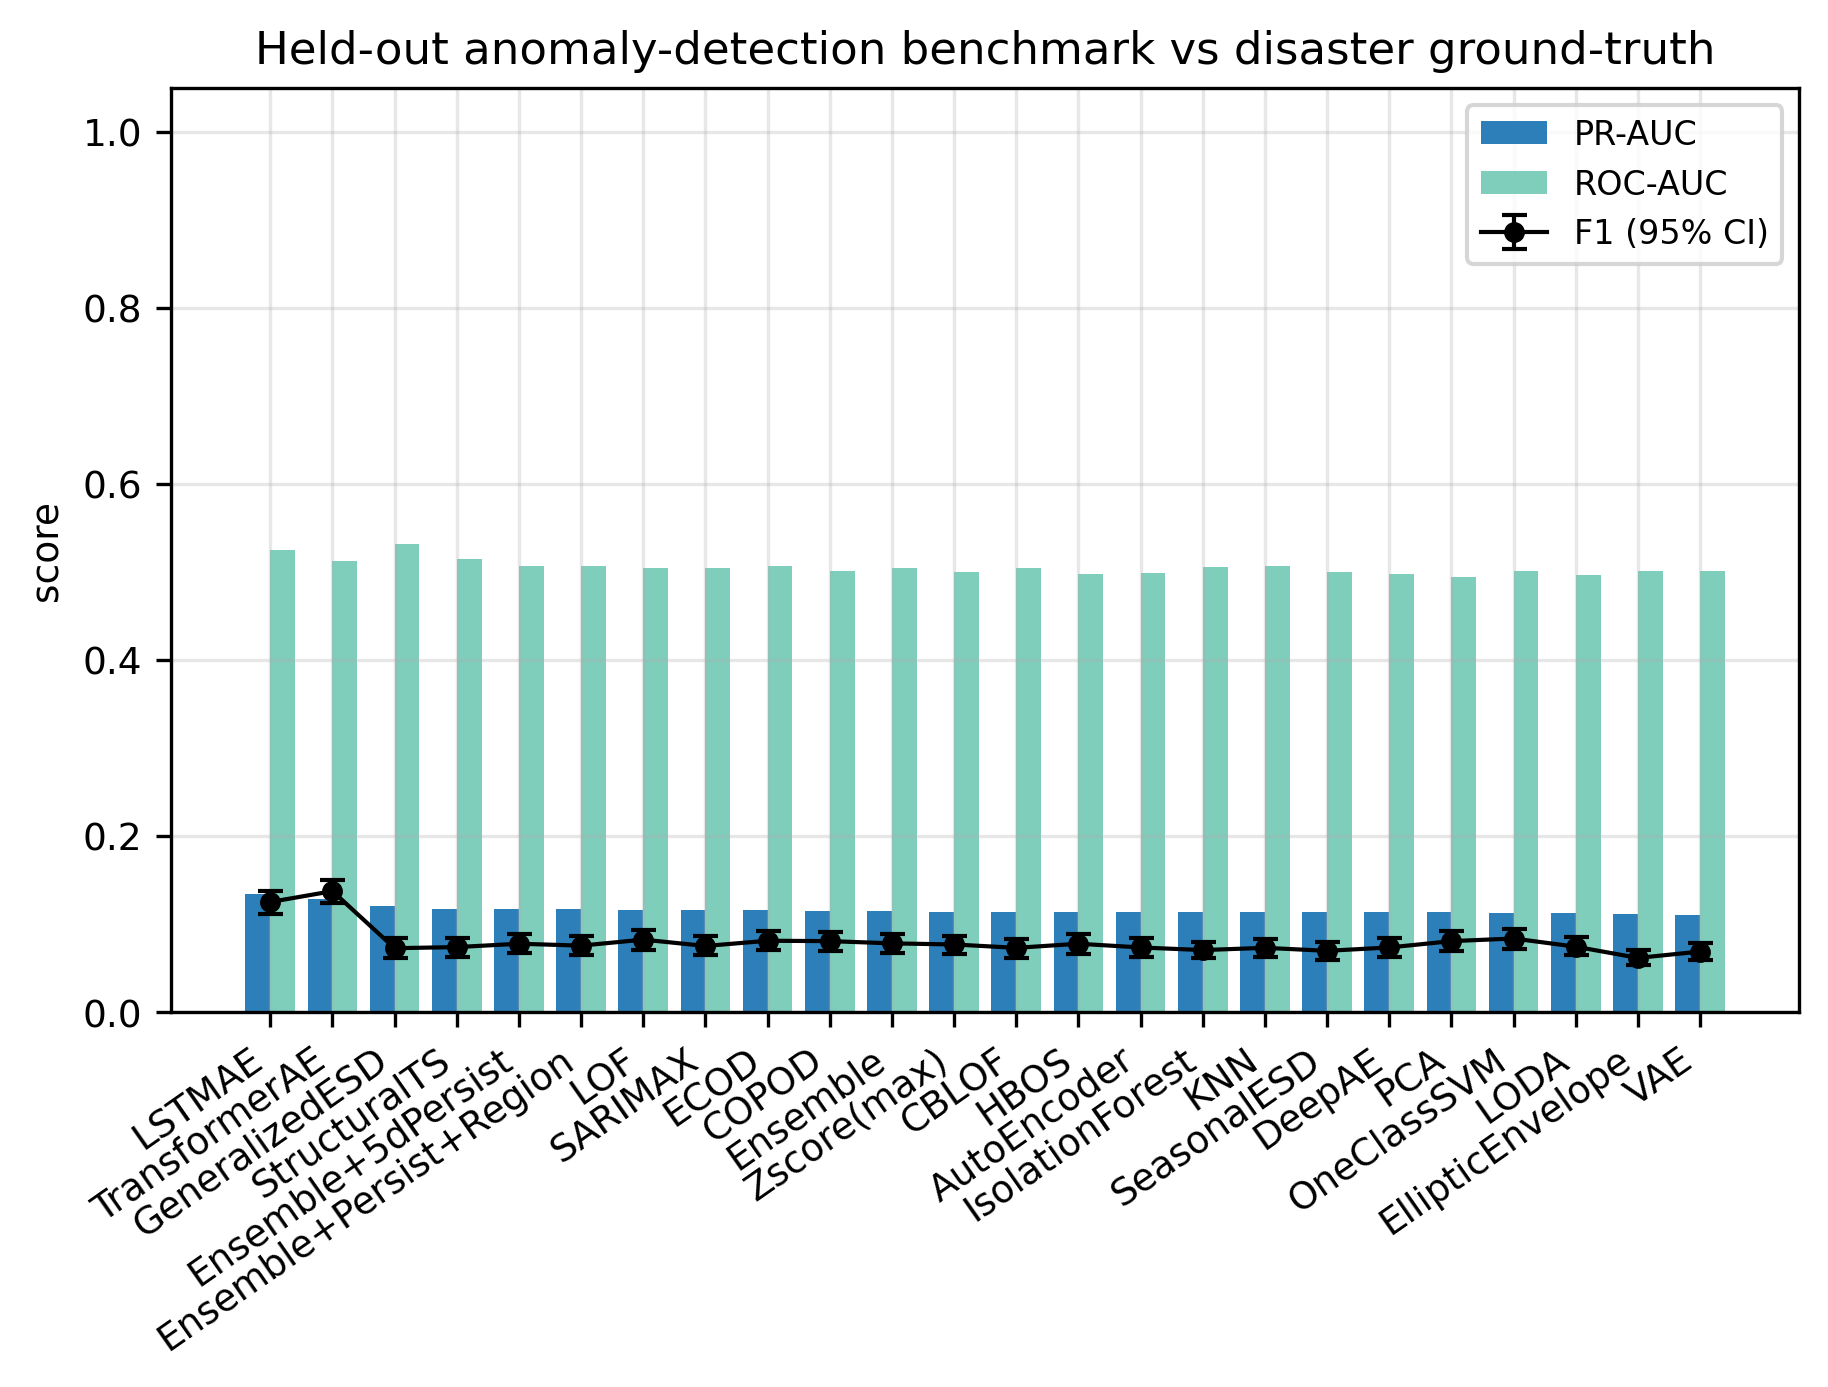
\includegraphics[width=\linewidth]{figures/fig_benchmark.png}
\caption{Held-out detector benchmark. The cross-sectional methods cluster at
chance; only the two torch sequence autoencoders (LSTM-AE, Transformer-AE) rise
slightly above the size-matched random null on F1/PR-AUC while still ranking near
chance on ROC-AUC. F1 error bars are 95\% bootstrap intervals. (RQ1)}
\label{fig:benchmark}
\end{figure}
\begin{figure}[h]\centering
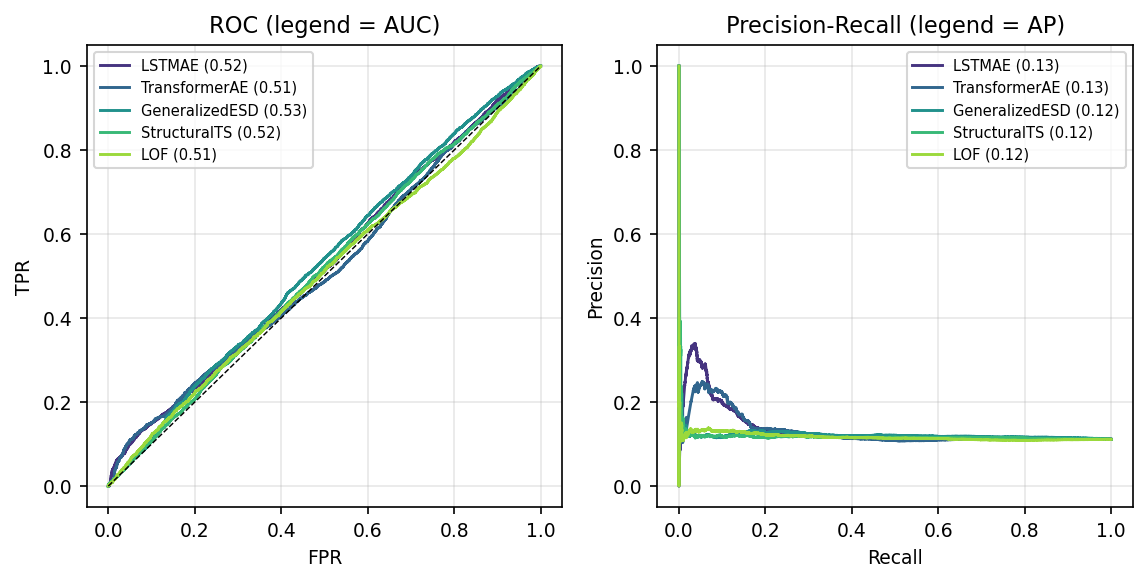
\includegraphics[width=\linewidth]{figures/fig_roc_pr.png}
\caption{ROC and precision--recall curves for top detectors; ROC hugs the
diagonal, PR barely exceeds the base-rate line. (RQ1)}
\label{fig:curves}
\end{figure}
\begin{figure}[h]\centering
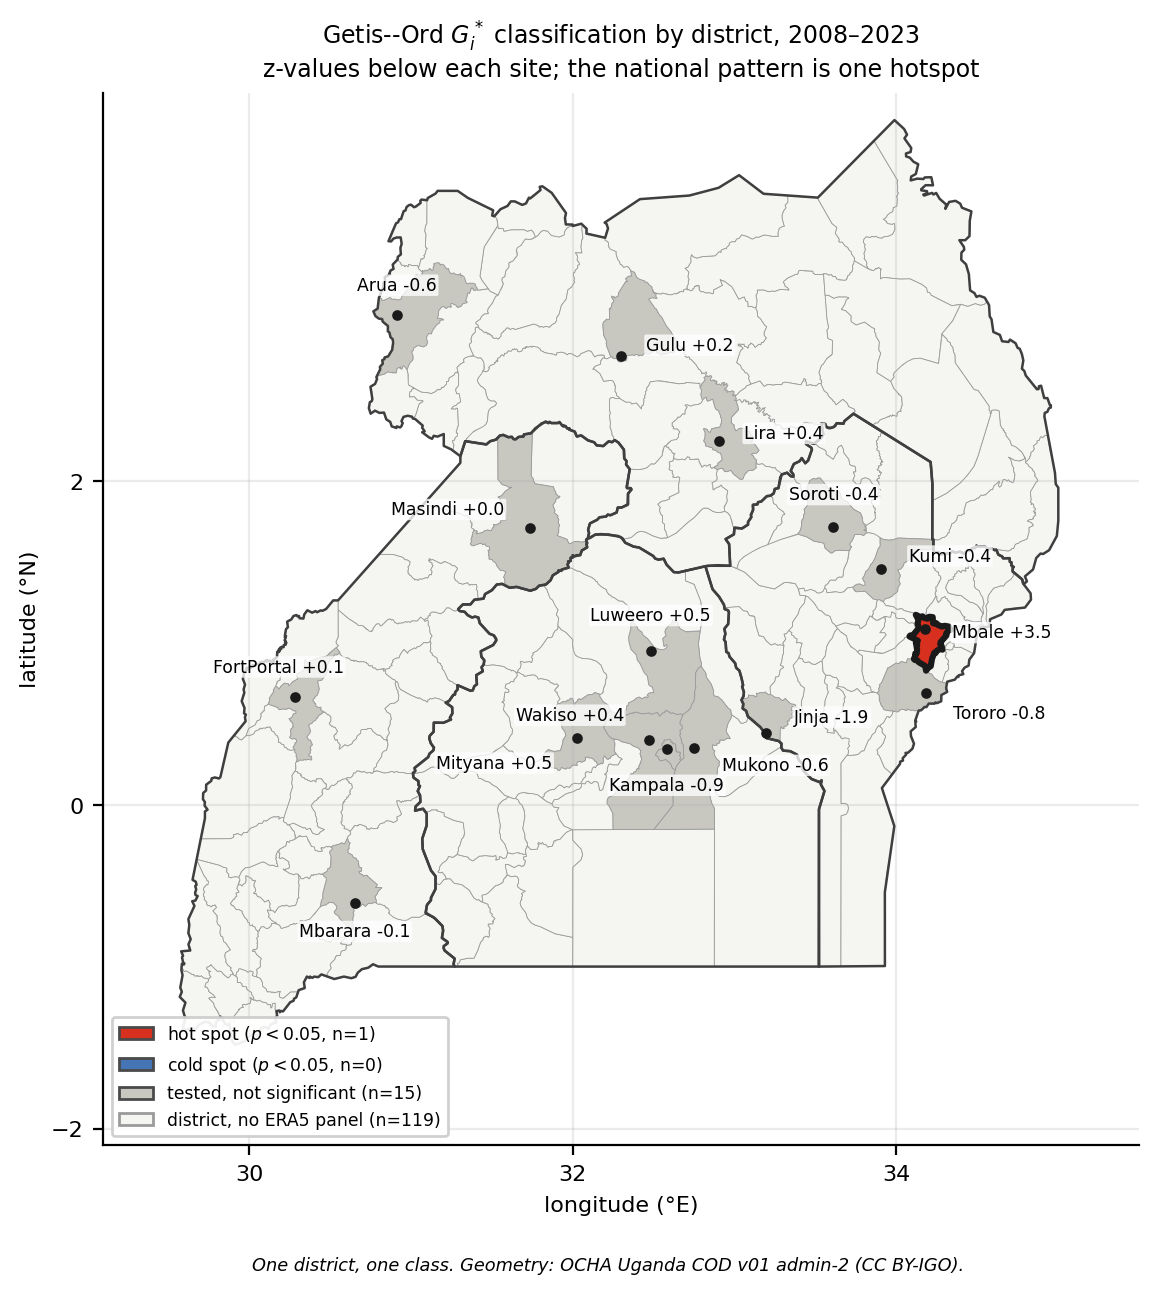
\includegraphics[width=\linewidth]{figures/fig_hotspot_map.png}
\caption{Getis--Ord $G_i^*$ classification drawn as a district choropleth: one
significant hotspot (Mbale, $z=3.50$), no significant coldspot, 15 districts
tested and not significant, and 119 districts the ERA5 panel does not observe.
The $z$-value is printed beside each observation point and thick internal lines
are the four administrative regions. Geometry: OCHA Uganda COD
v01 admin-2 (CC BY-IGO). (RQ2)}
\label{fig:map}
\end{figure}
\begin{figure}[h]\centering
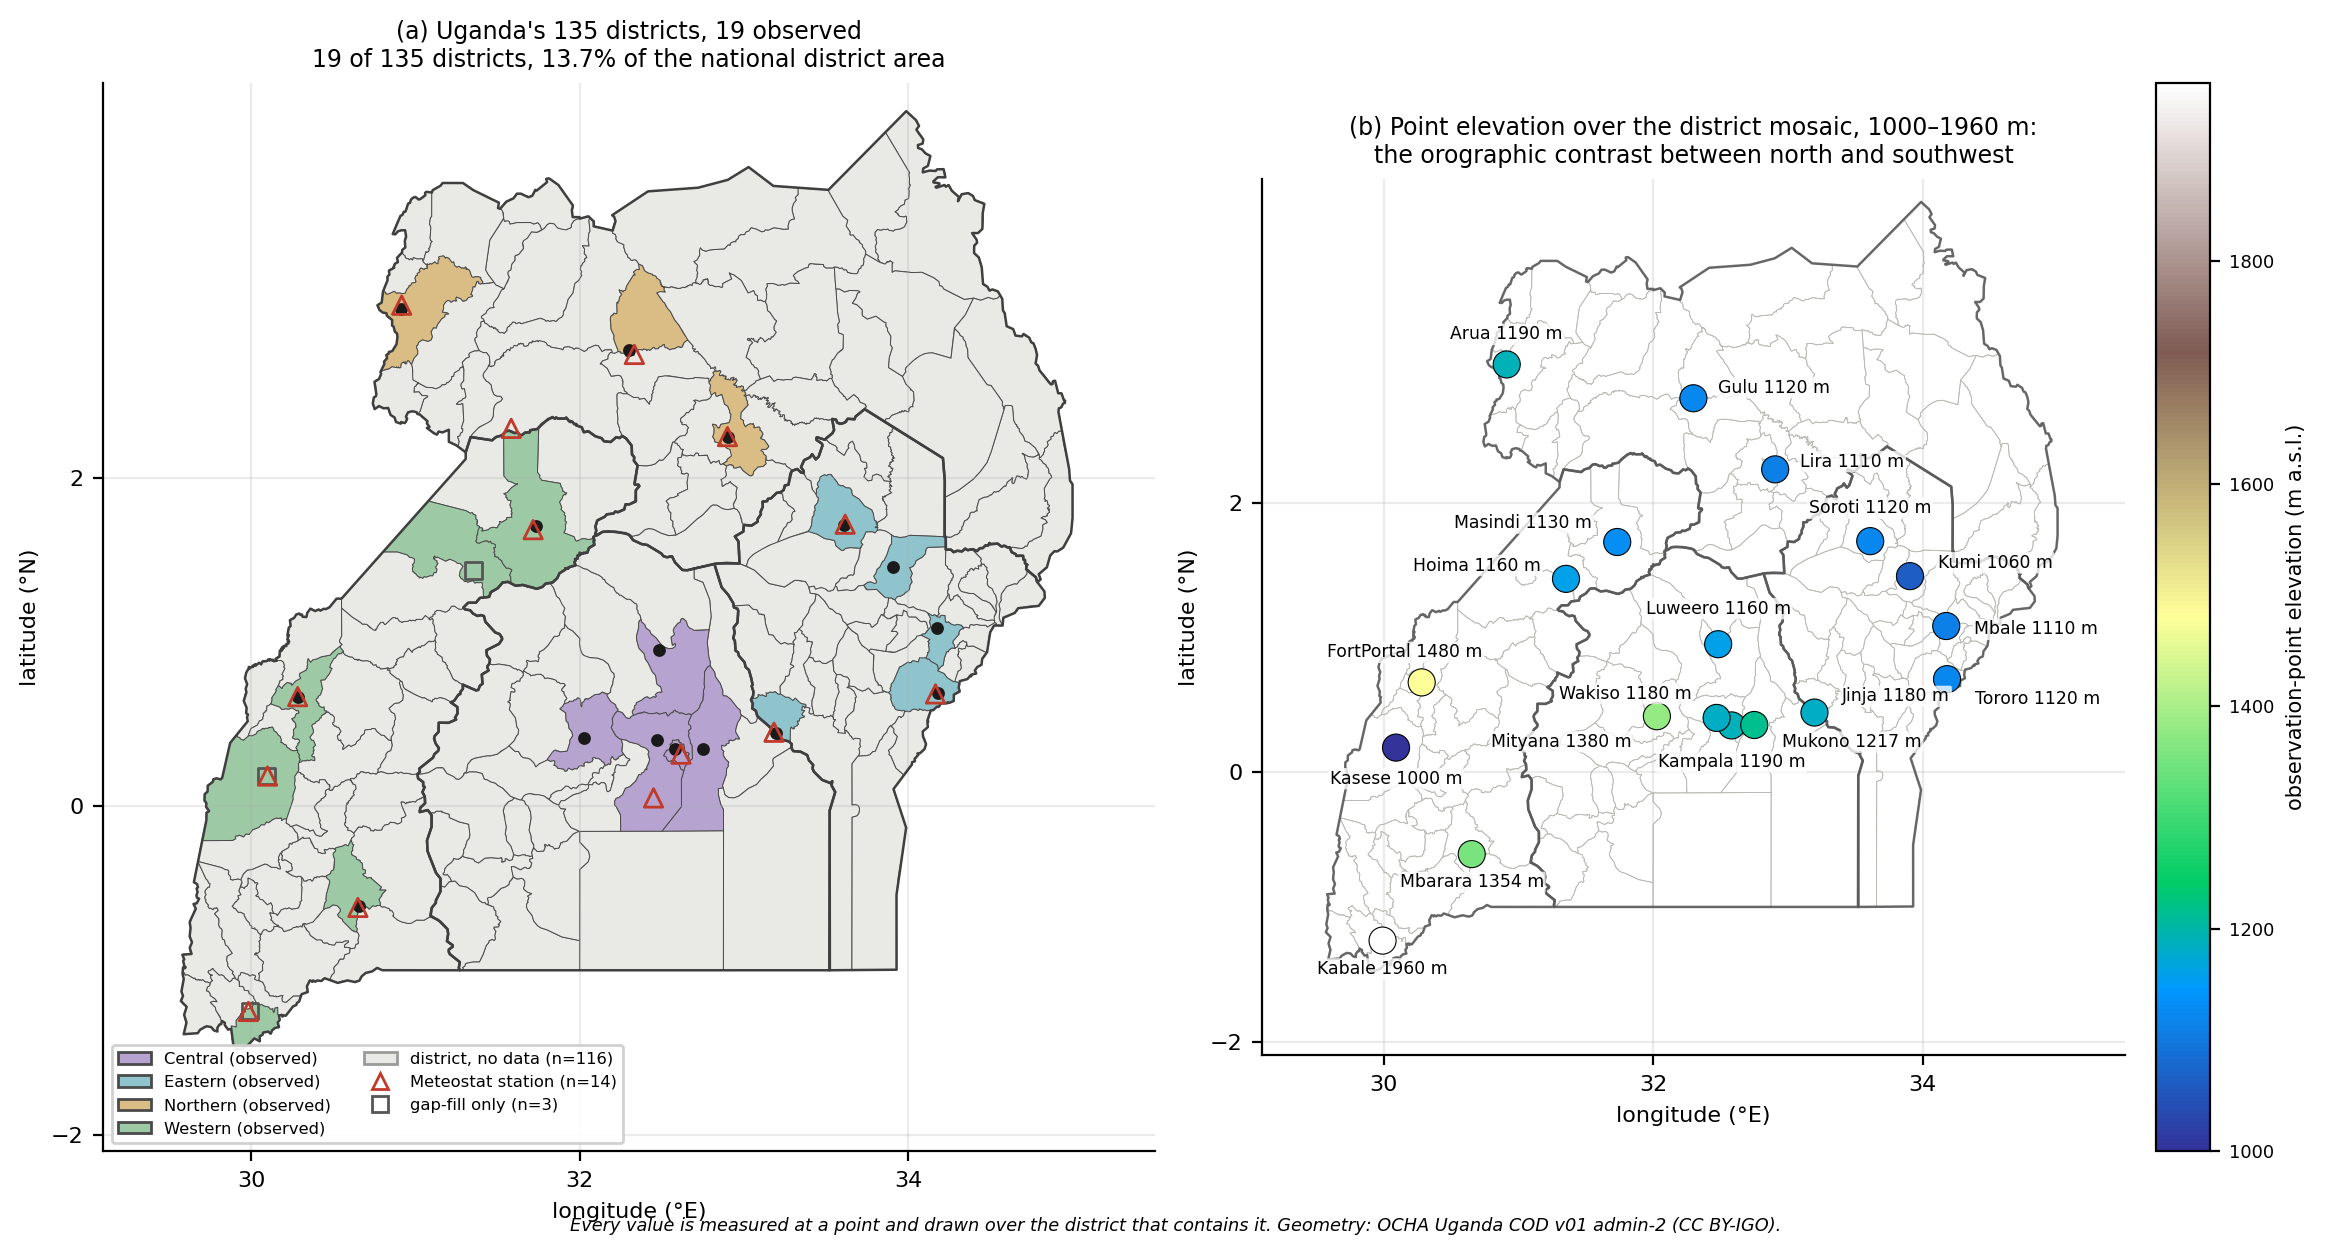
\includegraphics[width=\linewidth]{figures/fig_study_area.png}
\caption{Reference geometry of the three observation substrates, drawn on the
135-district administrative mosaic of the OCHA Uganda COD (CC BY-IGO). Left:
districts shaded by the region that contains an observation point, with the 16
ERA5 sites (dots), the Meteostat station network (14 locations, 12 of which
return data; triangles) and the three sites reachable only through the NASA
POWER gap-fill (squares); 116 districts carry no observation and are drawn as
no-data. Right: observation-point elevation over the same mosaic, showing the
orographic contrast between the northern and south-western sites. Each value is
measured at a point and shaded over the district that contains it; no areal
average is implied. (Data)}
\label{fig:studyarea}
\end{figure}
\begin{figure}[h]\centering
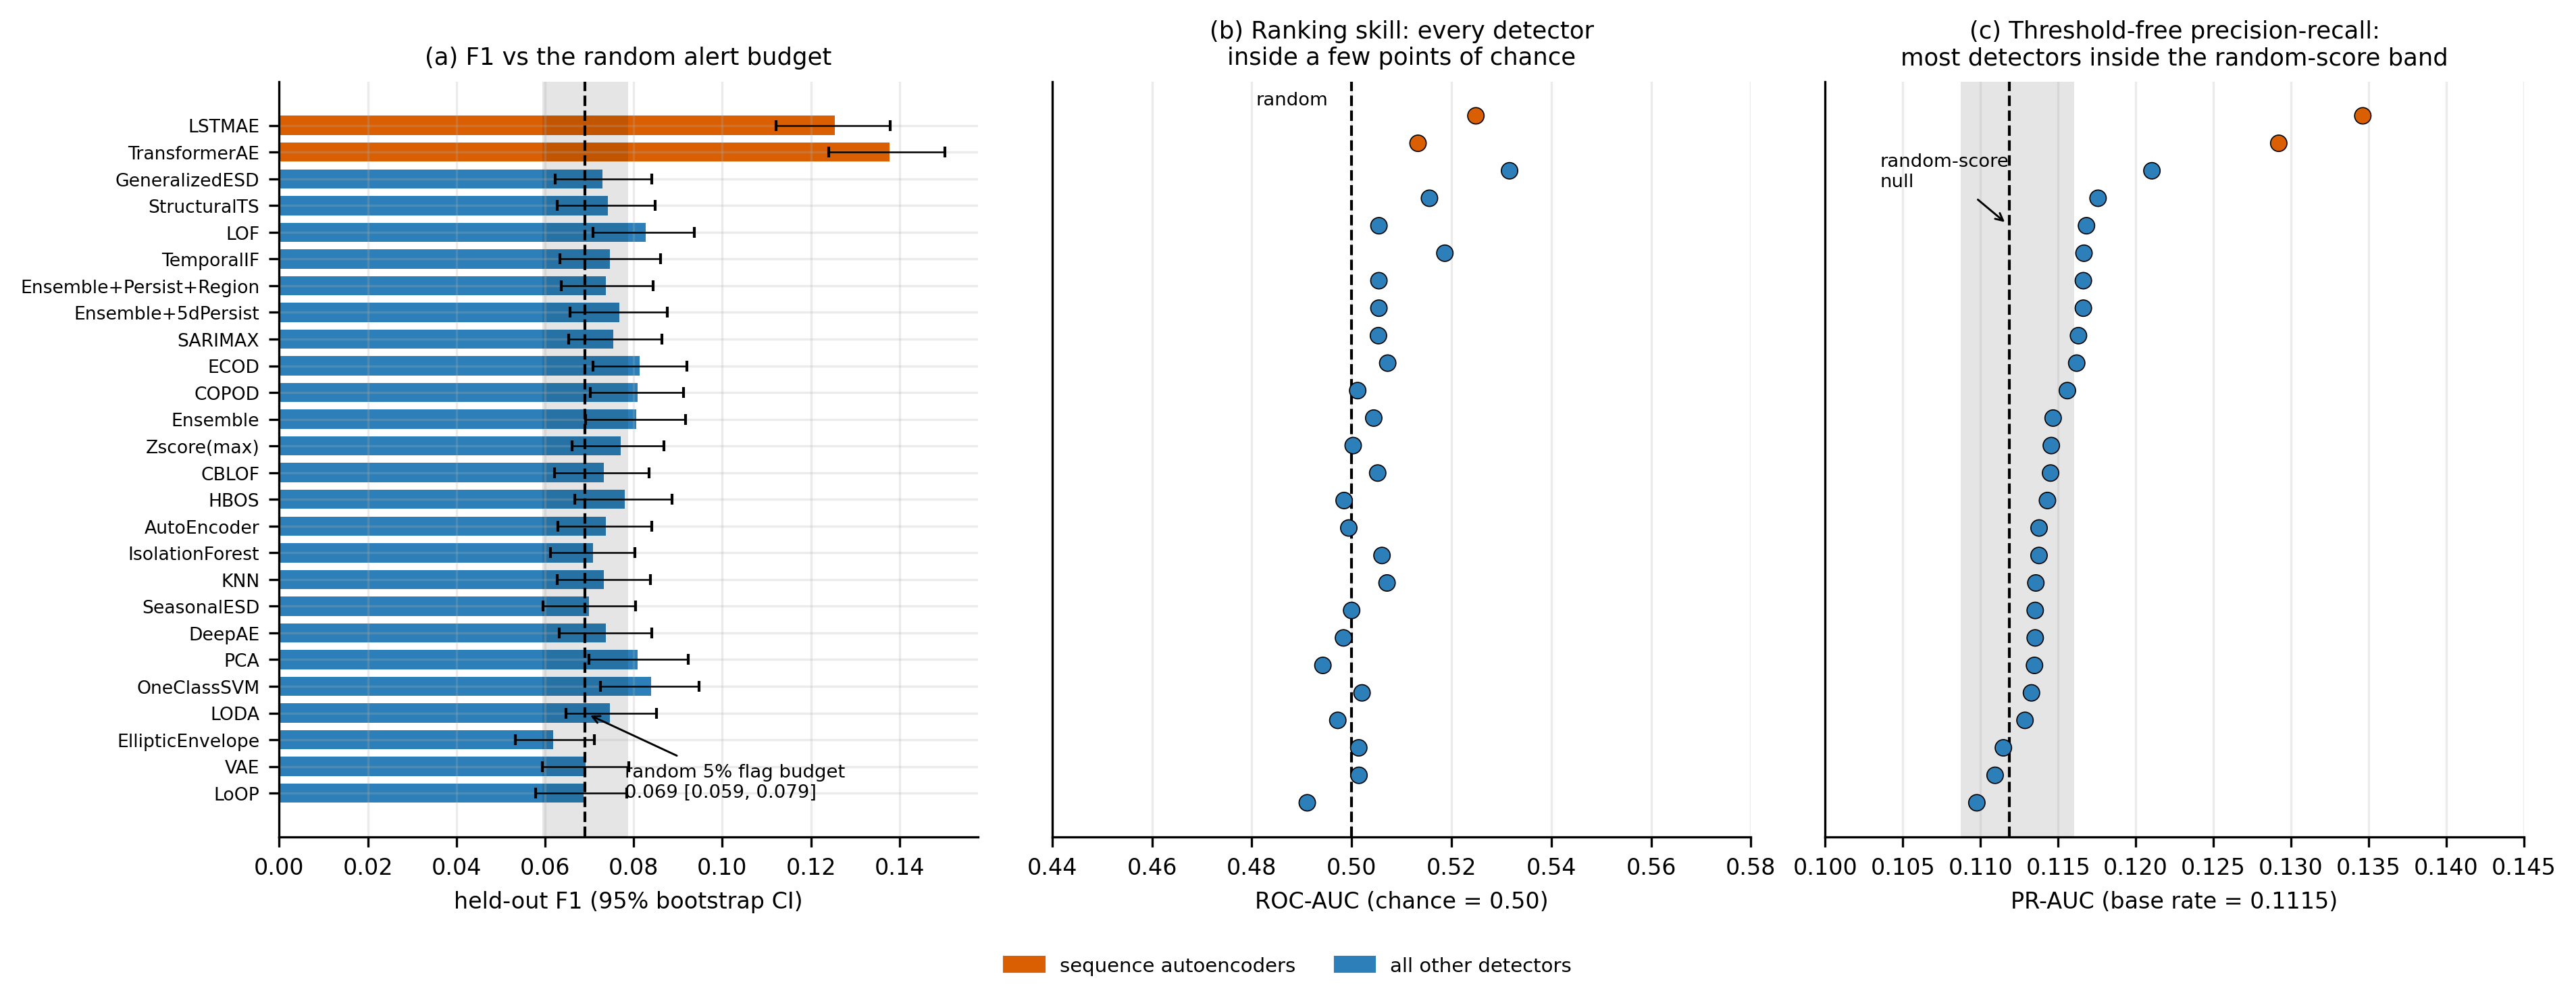
\includegraphics[width=\linewidth]{figures/fig_null_comparison.png}
\caption{The negative result made legible by zooming onto the reference values.
(a) Held-out F1 with 95\% bootstrap intervals against the random 5\% alert
budget ($0.069$, shaded Monte-Carlo interval $0.059$--$0.079$): the
cross-sectional detectors lie within $1.22\times$ of that mean, the two sequence
autoencoders near $2\times$. (b) ROC-AUC on an axis centred on chance: all 24
methods fall between 0.494 and 0.532. (c) PR-AUC against the random-score null
($0.112$, band $0.109$--$0.116$), which coincides with the base rate. (RQ1)}
\label{fig:null}
\end{figure}
\begin{figure}[h]\centering
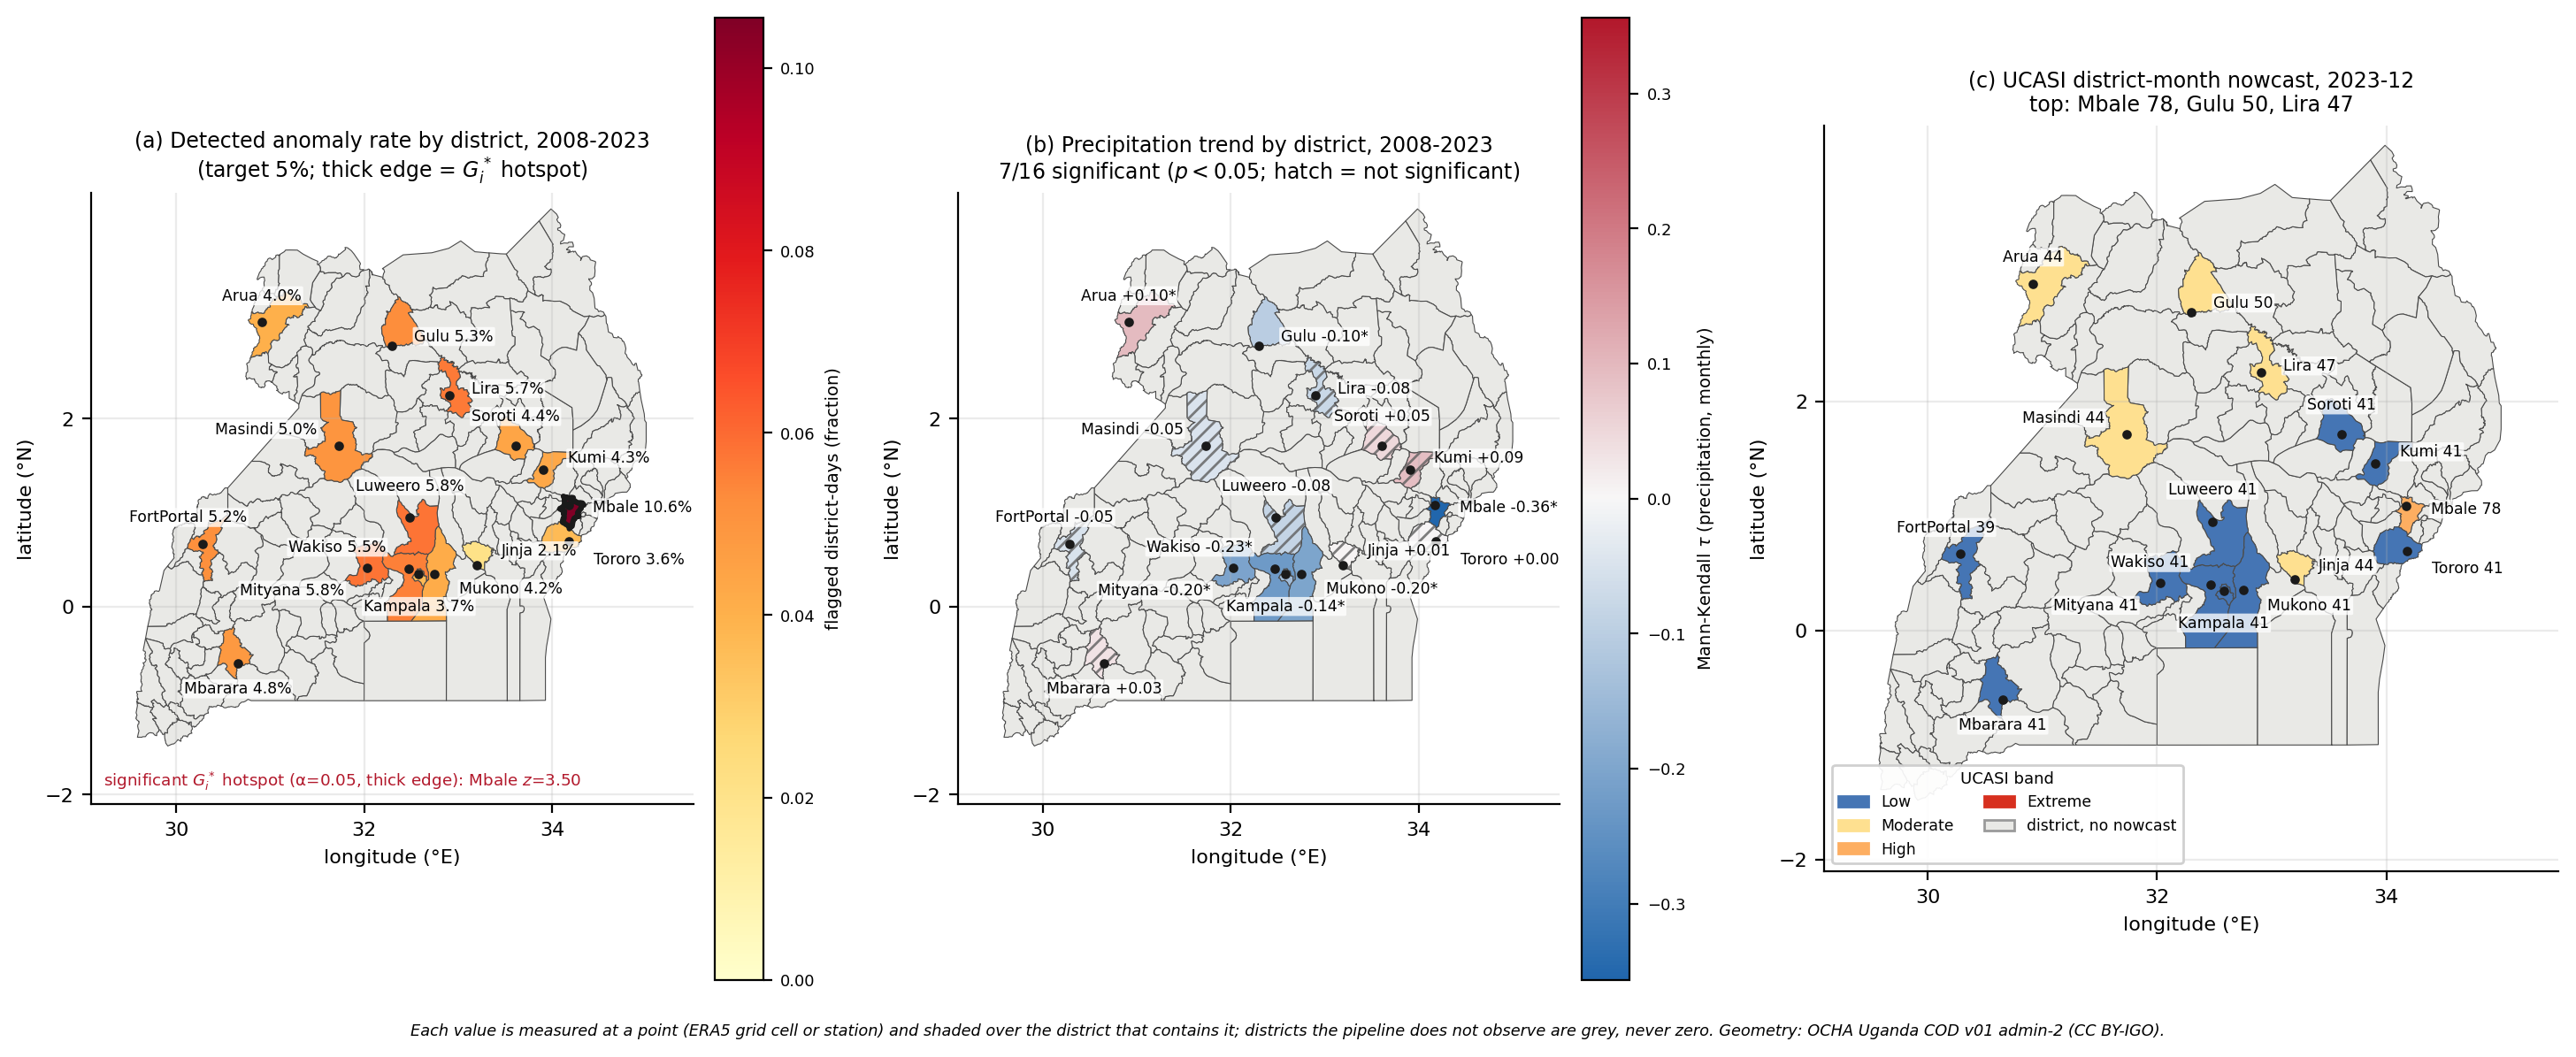
\includegraphics[width=\linewidth]{figures/fig_risk_maps.png}
\caption{District risk maps, all drawn from persisted artefacts on the OCHA
Uganda COD admin-2 geometry (CC BY-IGO). (a) Detected anomaly rate 2008--2023
against the 5\% target, with the single significant Getis--Ord $G_i^*$ hotspot
(Mbale, $z=3.50$) outlined in black. (b) Mann--Kendall $\tau$ of monthly
precipitation by district, hatched where $p\geq0.05$; the Mbale drying is the
strongest negative coefficient. (c) UCASI district-month nowcast for the most
recent month in the surface (2023-12), banded by severity. Districts the panel
does not observe are grey in every panel, never zero. (RQ2, RQ4, RQ6)}
\label{fig:riskmaps}
\end{figure}
\begin{figure}[h]\centering
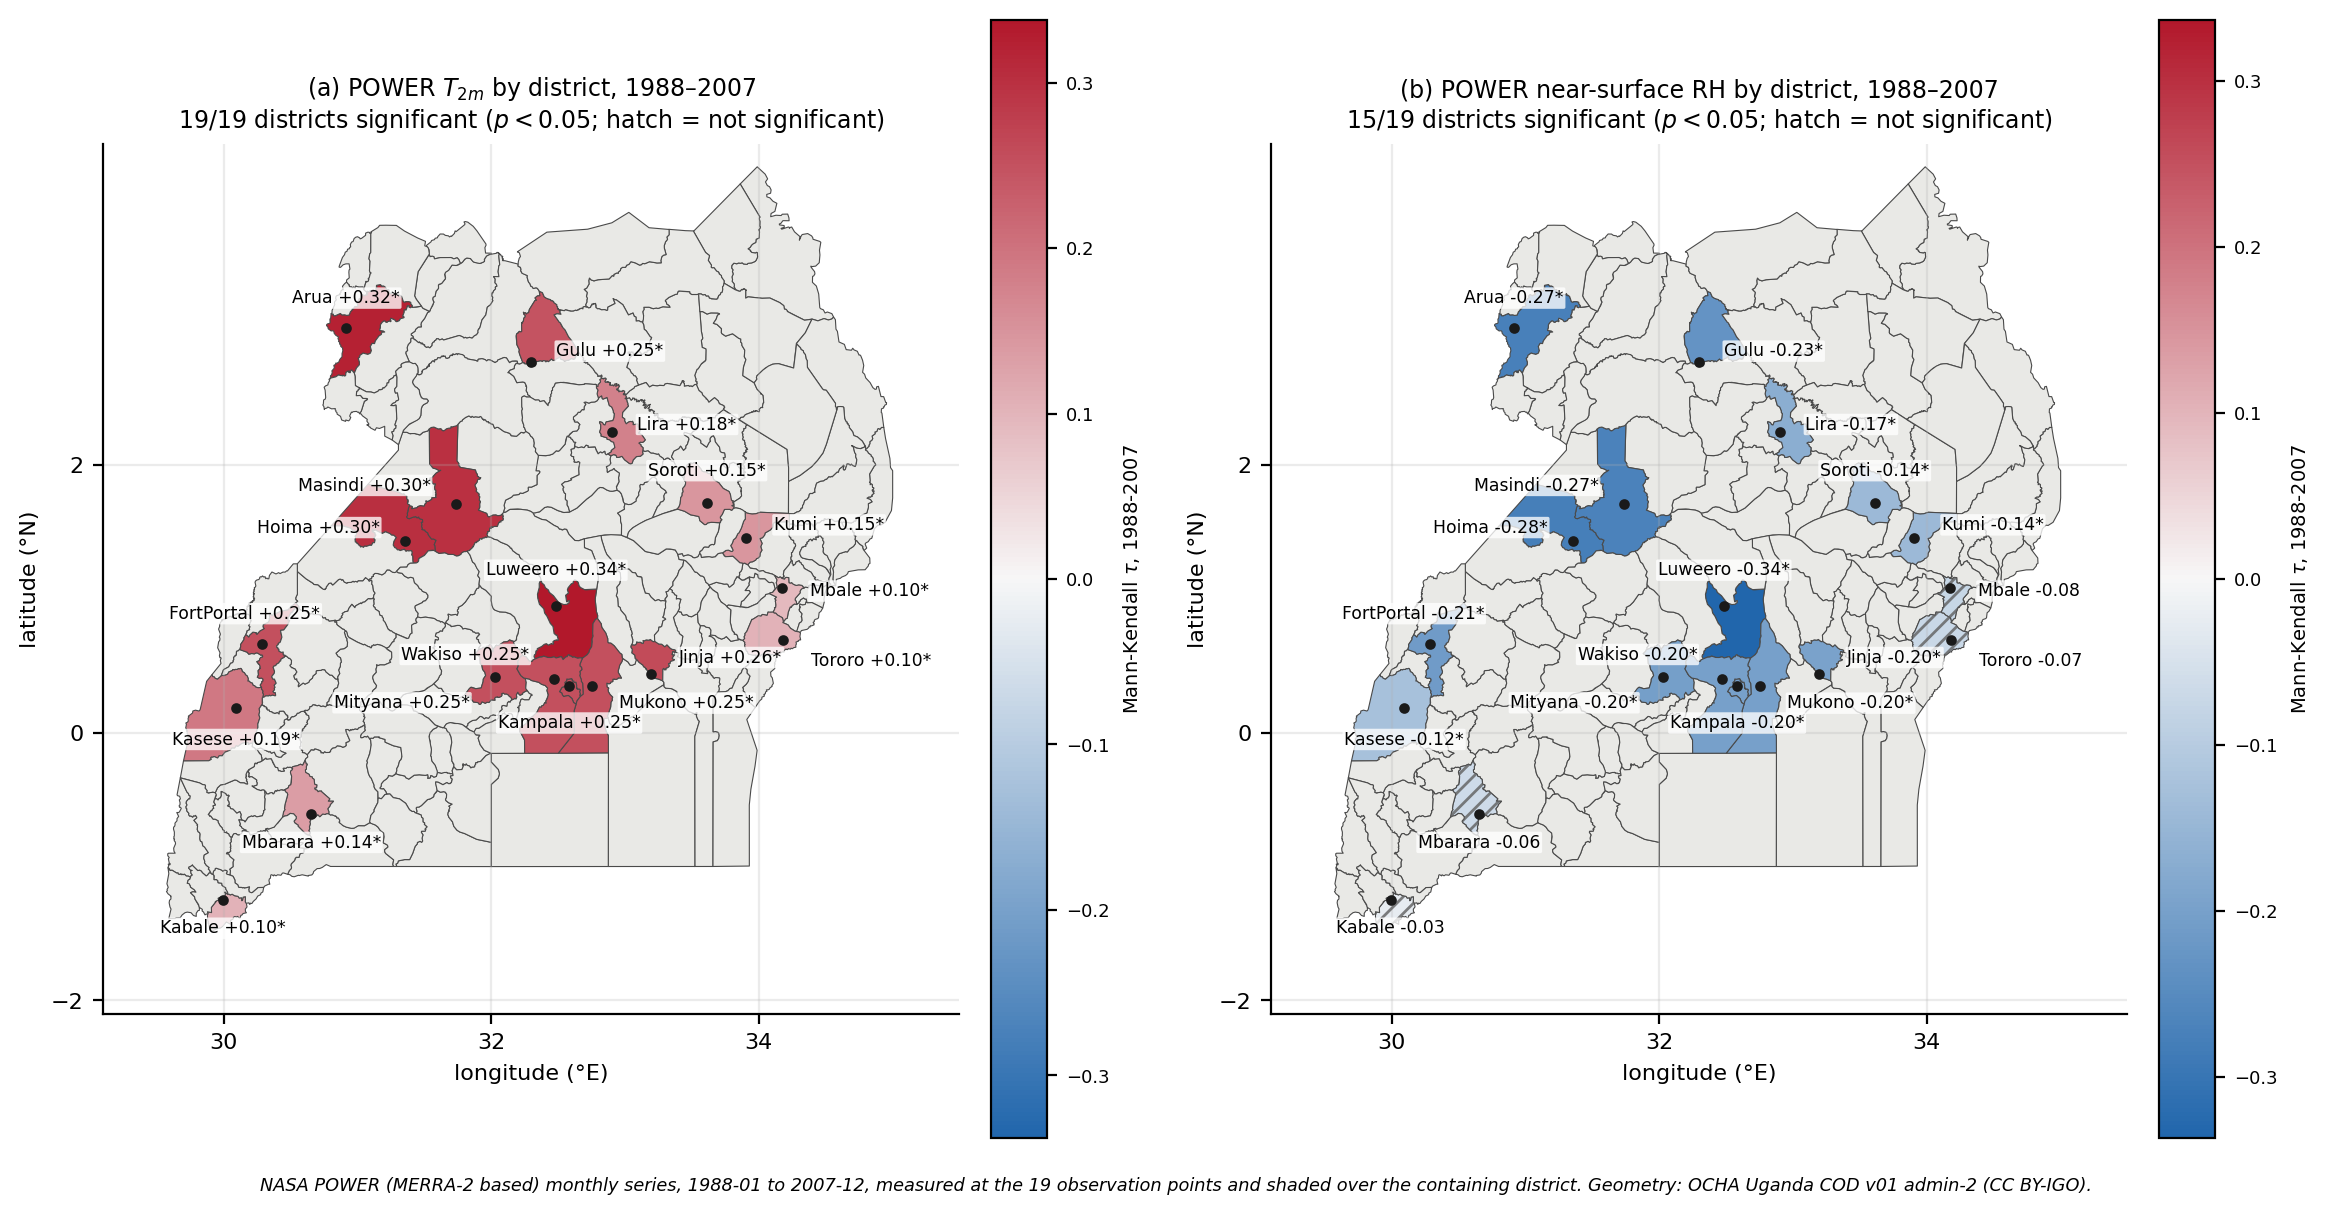
\includegraphics[width=\linewidth]{figures/fig_gapfill_maps.png}
\caption{Independent gap-fill trends drawn as district choropleths.
Mann--Kendall $\tau$ over 1988--2007 from NASA POWER at all 19 observation
points: near-surface temperature (left) warms significantly in 19/19 districts,
relative humidity (right) declines significantly in 15/19. Values are printed to
two decimals, starred where $p<0.05$; districts are hatched where the trend is
not significant, and districts without an observation are grey. Geometry: OCHA
Uganda COD v01 admin-2 (CC BY-IGO). (Novel gap-fill)}
\label{fig:gapfillmaps}
\end{figure}
\begin{figure}[h]\centering
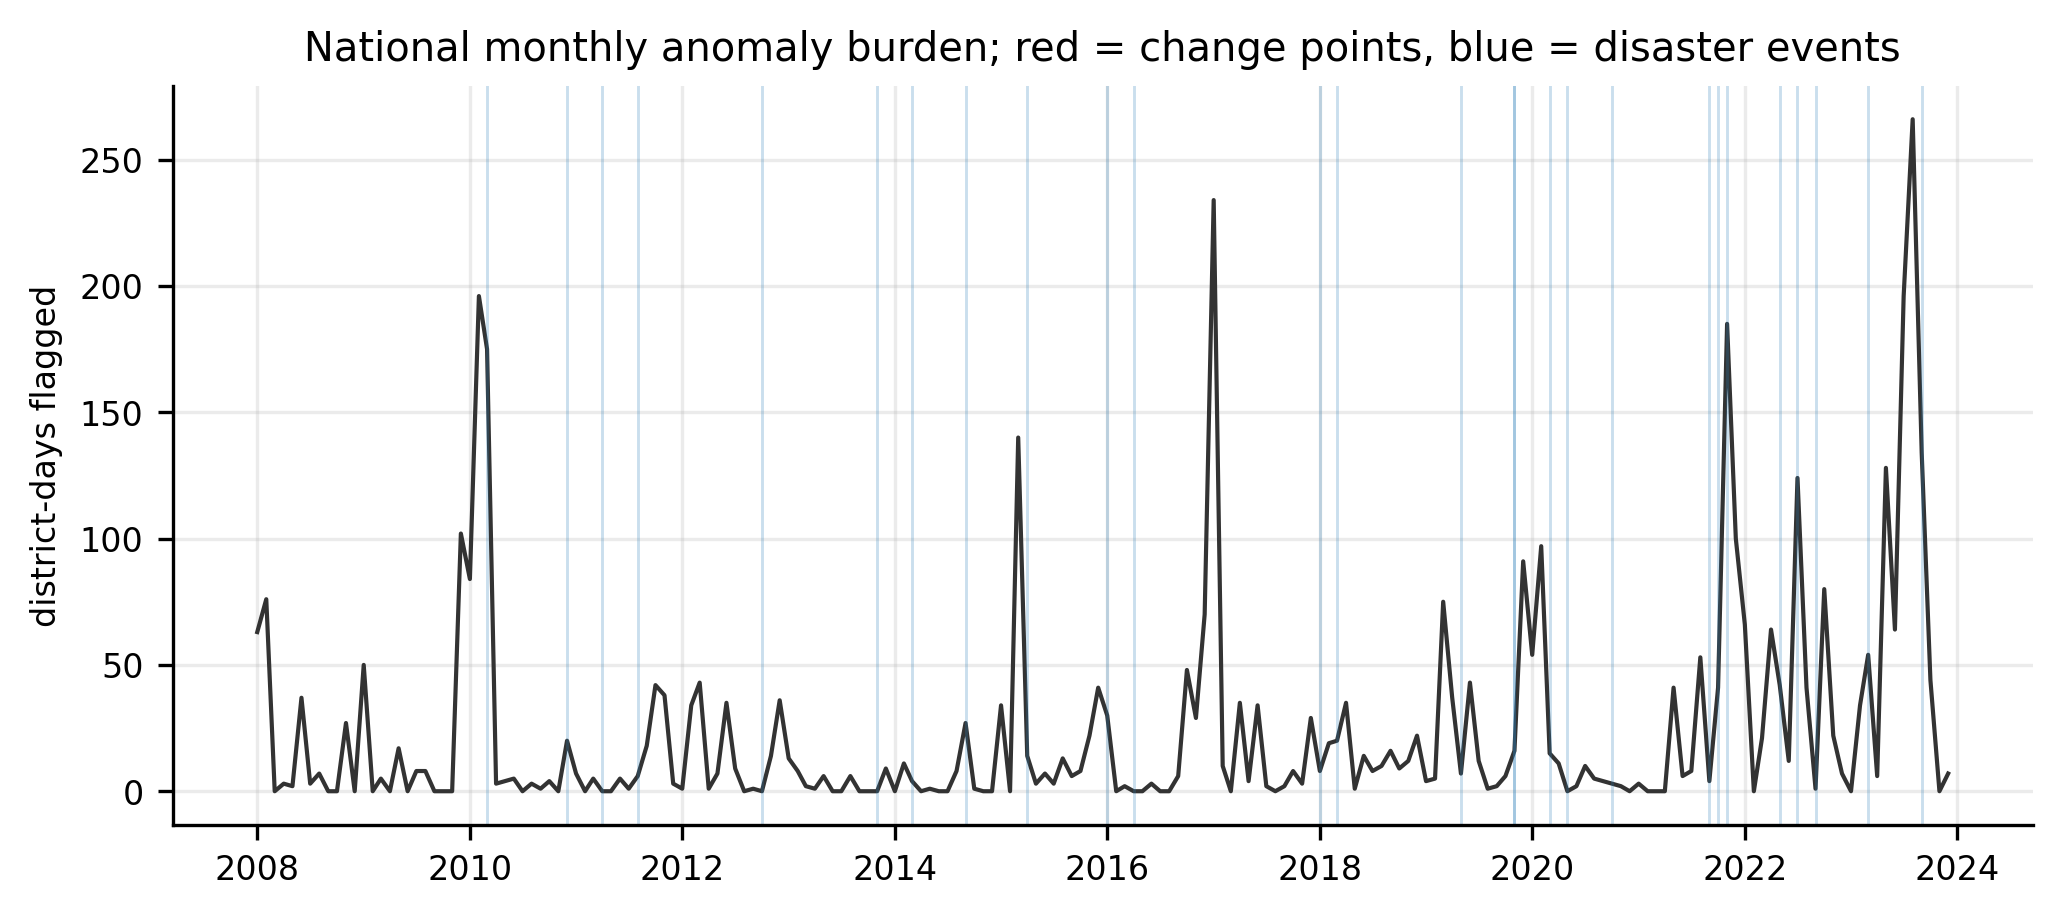
\includegraphics[width=\linewidth]{figures/fig_temporal.png}
\caption{National monthly anomaly burden with disaster-onset markers and
change-point screen. (RQ4)}
\label{fig:temporal}
\end{figure}
\begin{figure}[h]\centering
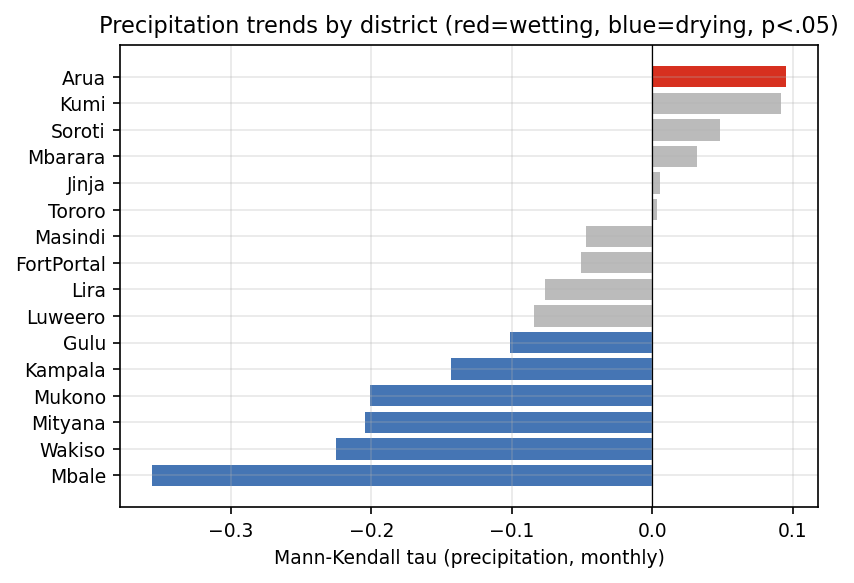
\includegraphics[width=0.8\linewidth]{figures/fig_mannkendall.png}
\caption{District-level precipitation Mann--Kendall $\tau$ (warming/drying
structure). (RQ4)}
\label{fig:mk}
\end{figure}
\begin{figure}[h]\centering
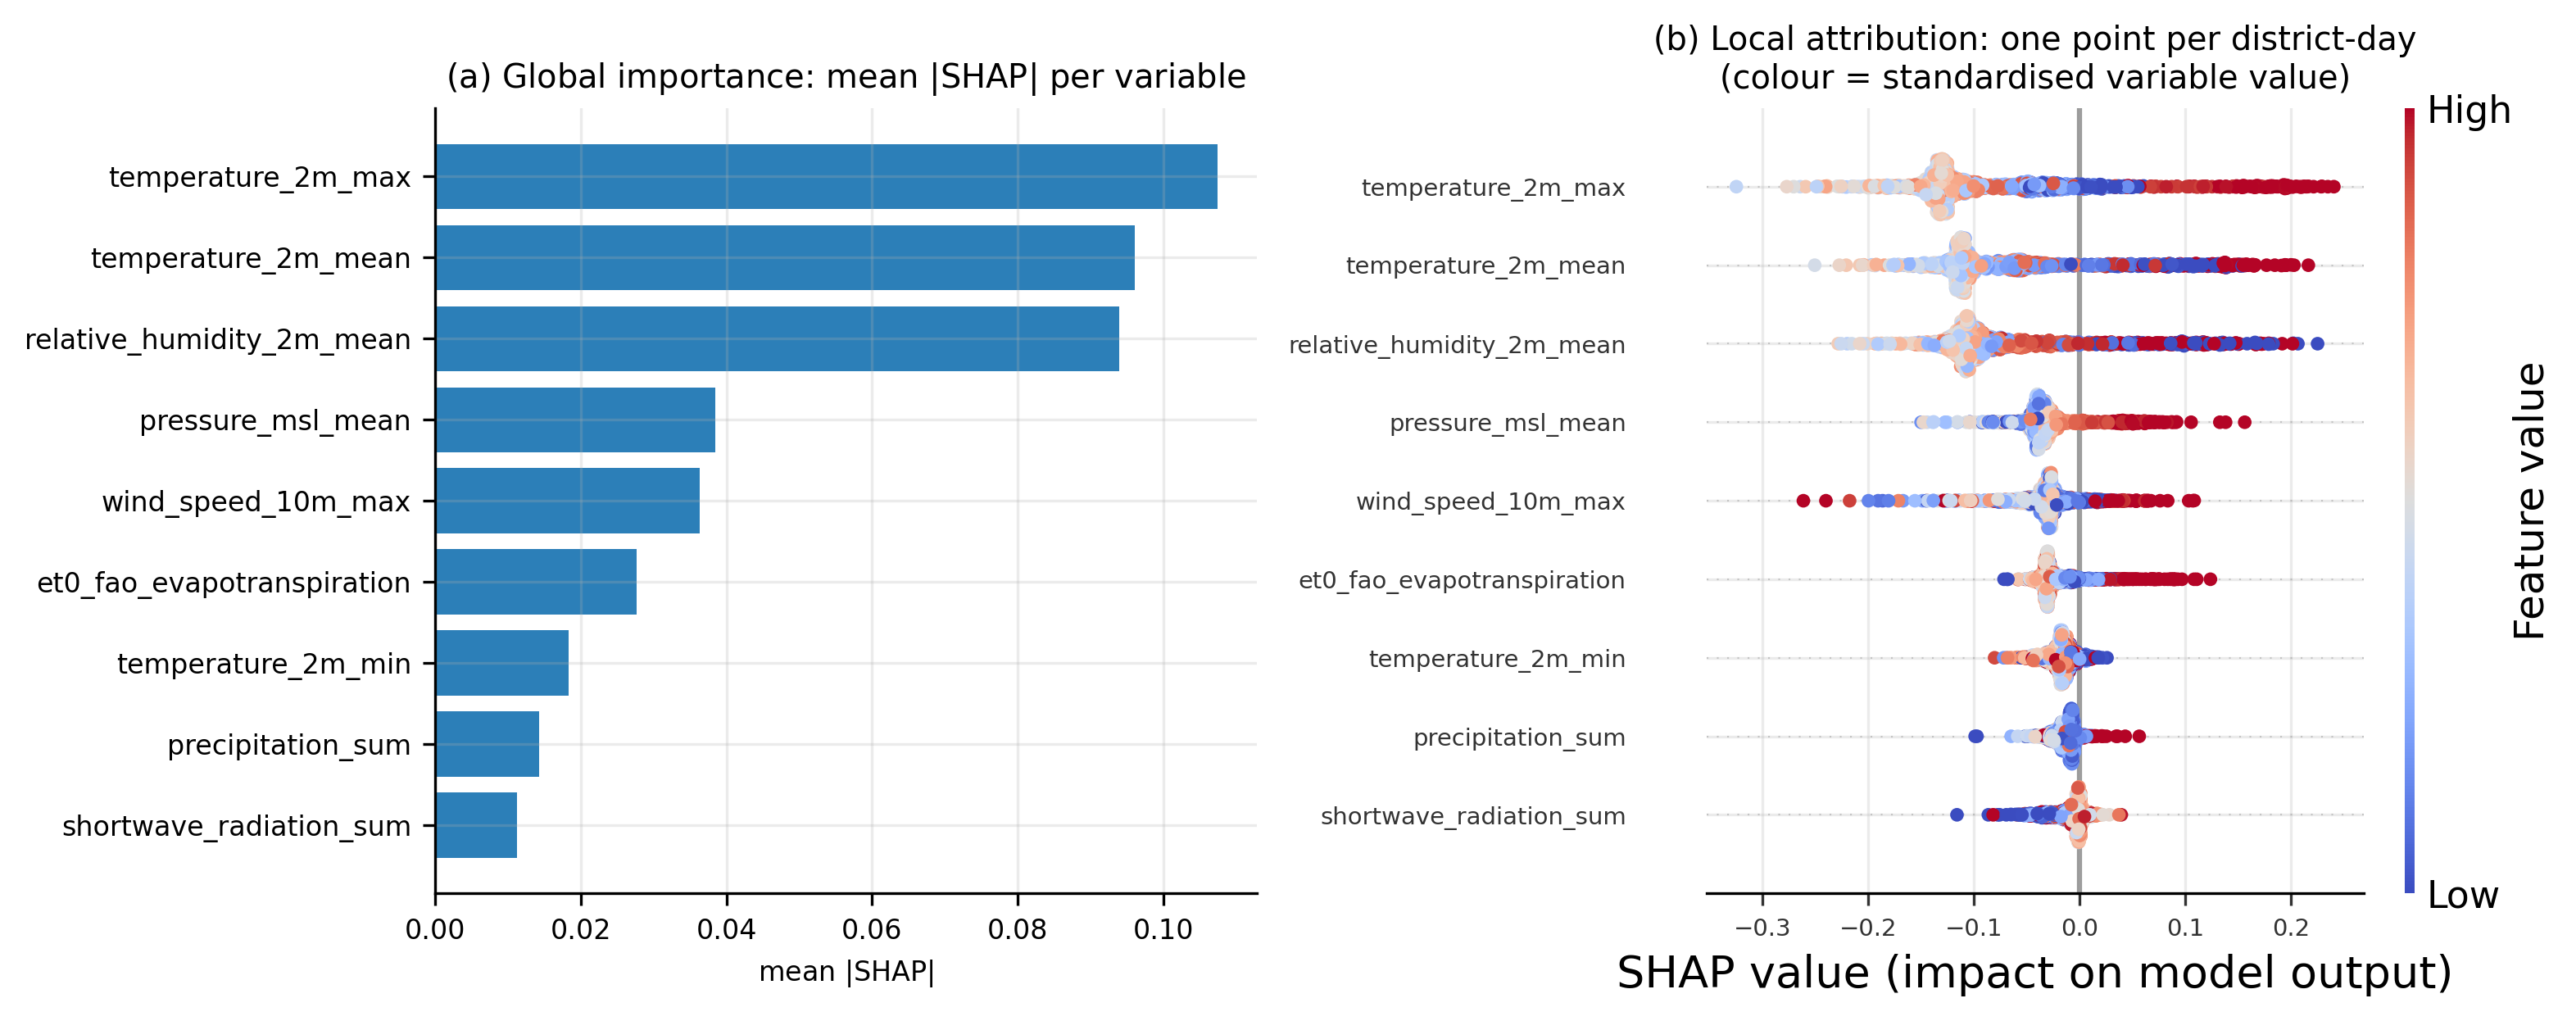
\includegraphics[width=0.8\linewidth]{figures/fig_shap.png}
\caption{SHAP global importance of weather features for the detection signal.
(RQ3)}
\label{fig:shap}
\end{figure}
\begin{figure}[h]\centering
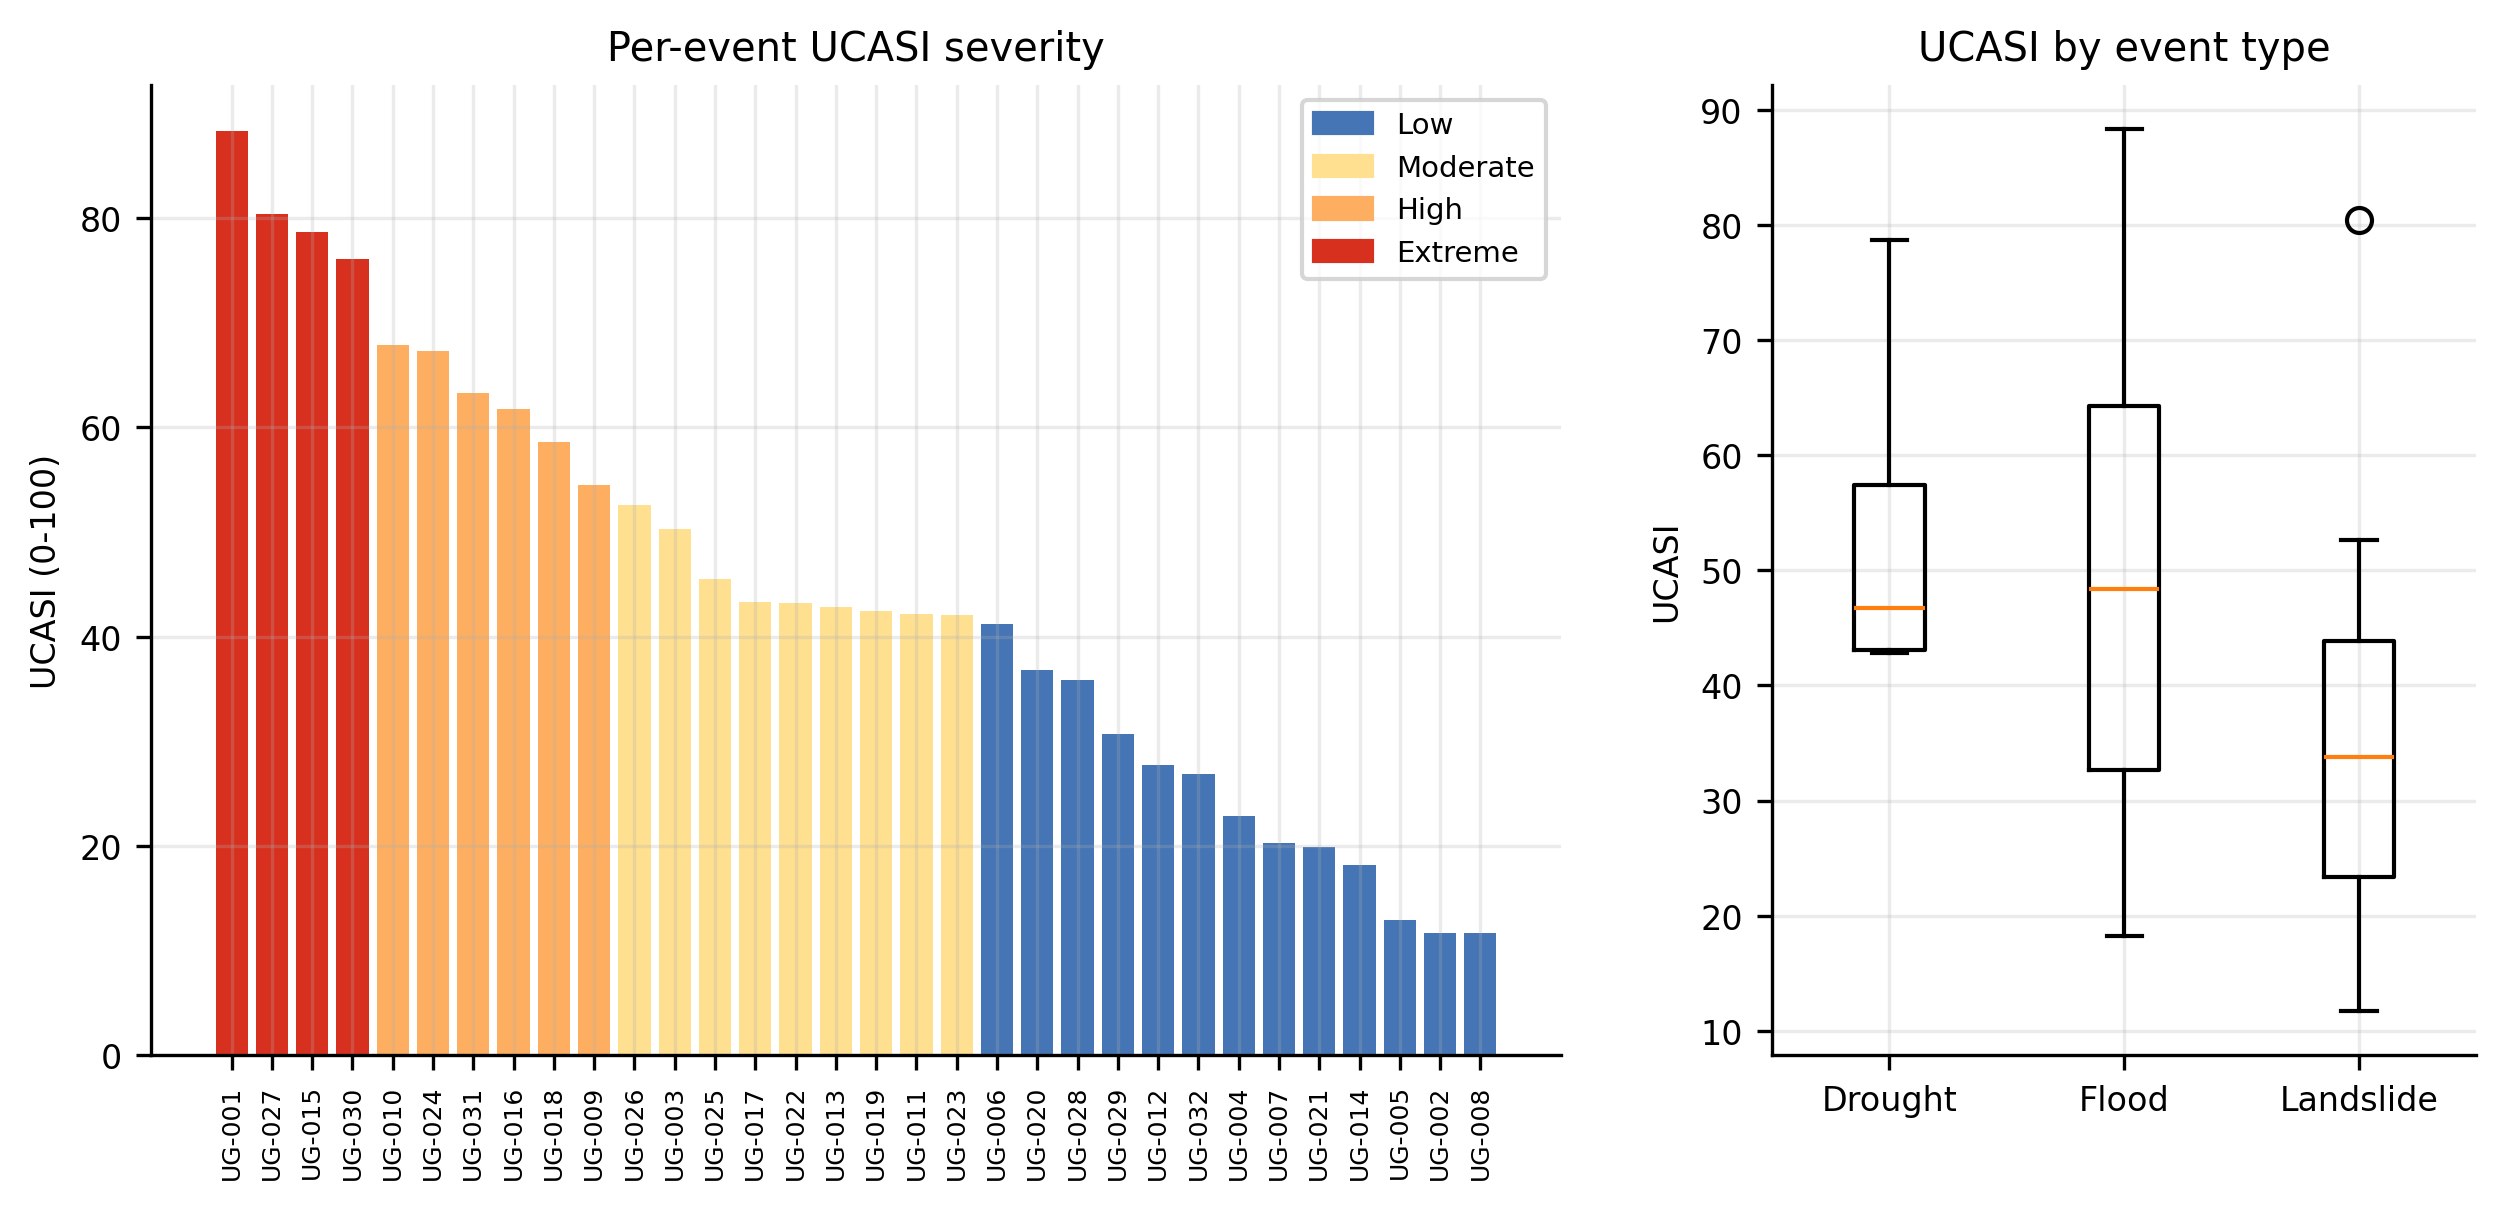
\includegraphics[width=\linewidth]{figures/fig_ucasi.png}
\caption{Per-event UCASI severity and distribution by hazard type. (Novel index)}
\label{fig:ucasi}
\end{figure}
\begin{figure}[h]\centering
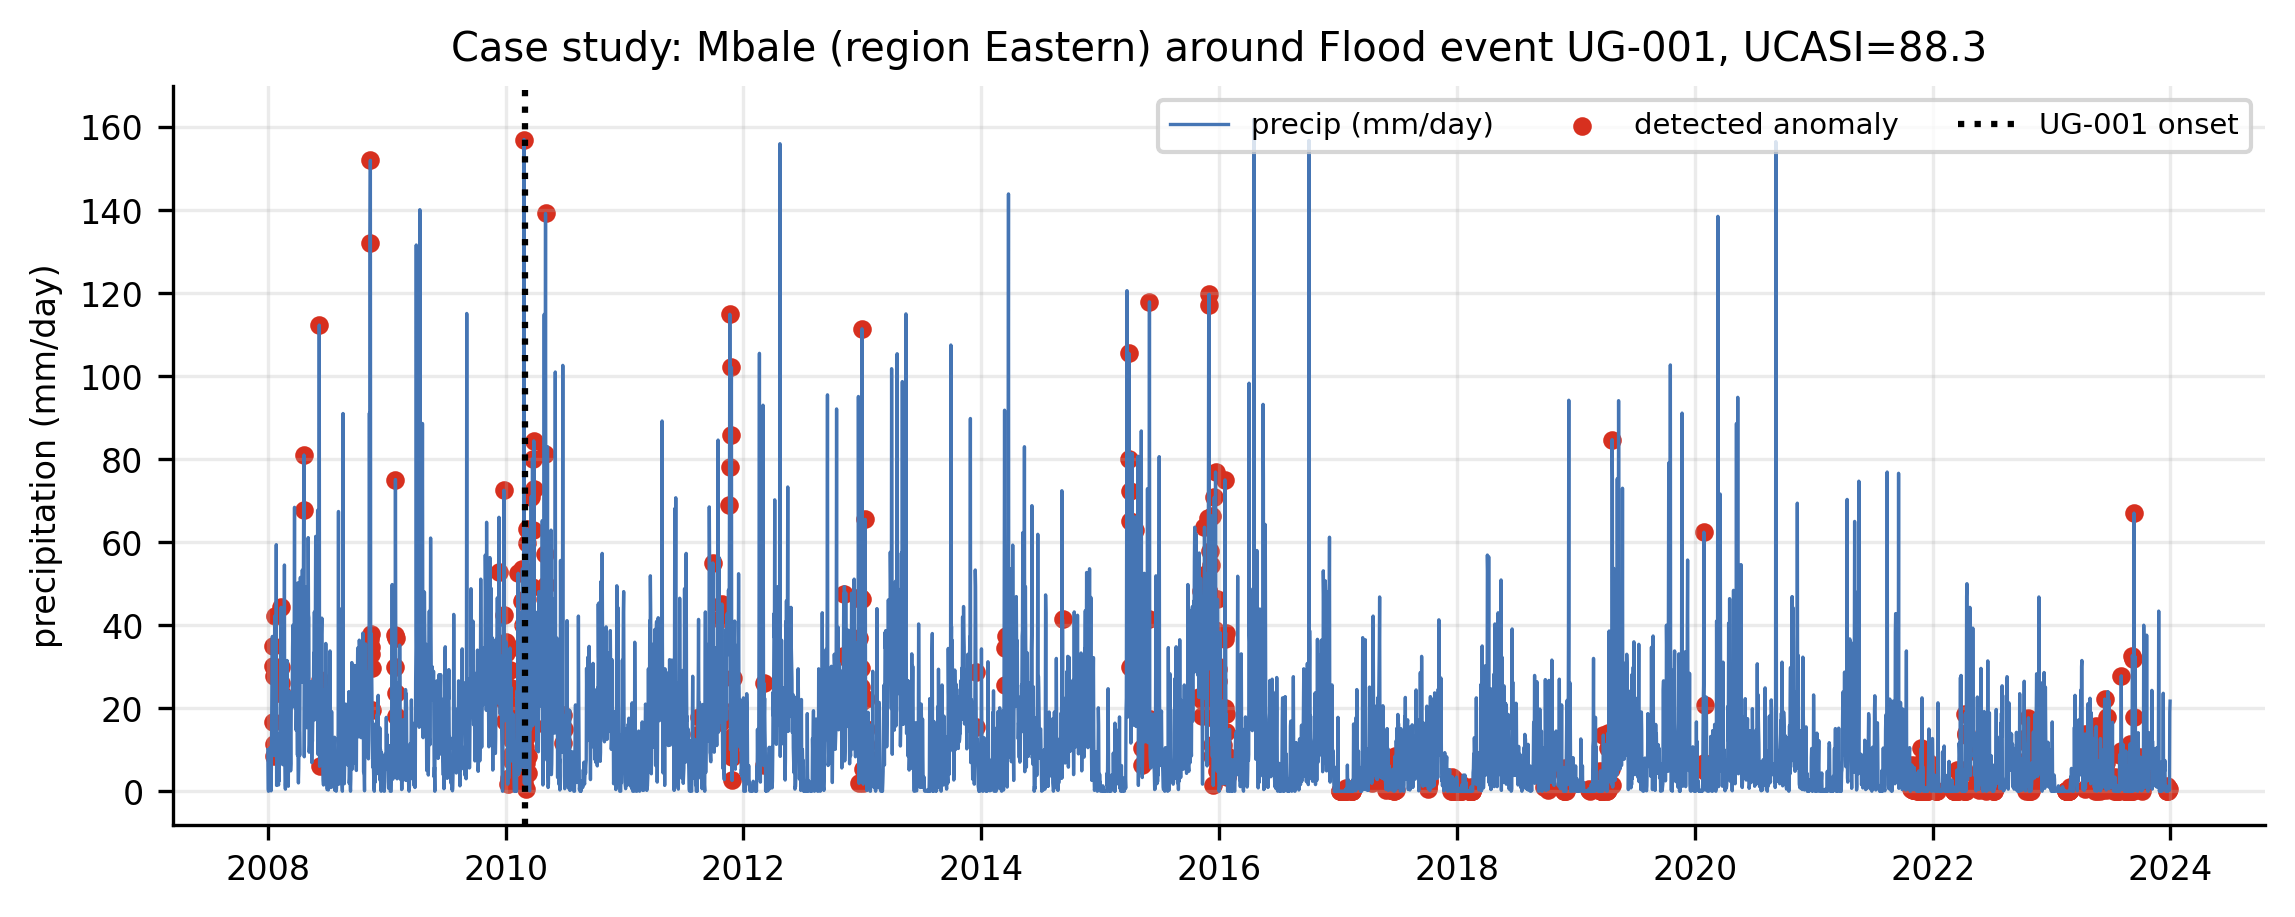
\includegraphics[width=\linewidth]{figures/fig_case_study.png}
\caption{Case study: daily precipitation and detected anomalies around the
top-ranked (2010) event.}
\label{fig:case}
\end{figure}
\begin{figure}[h]\centering
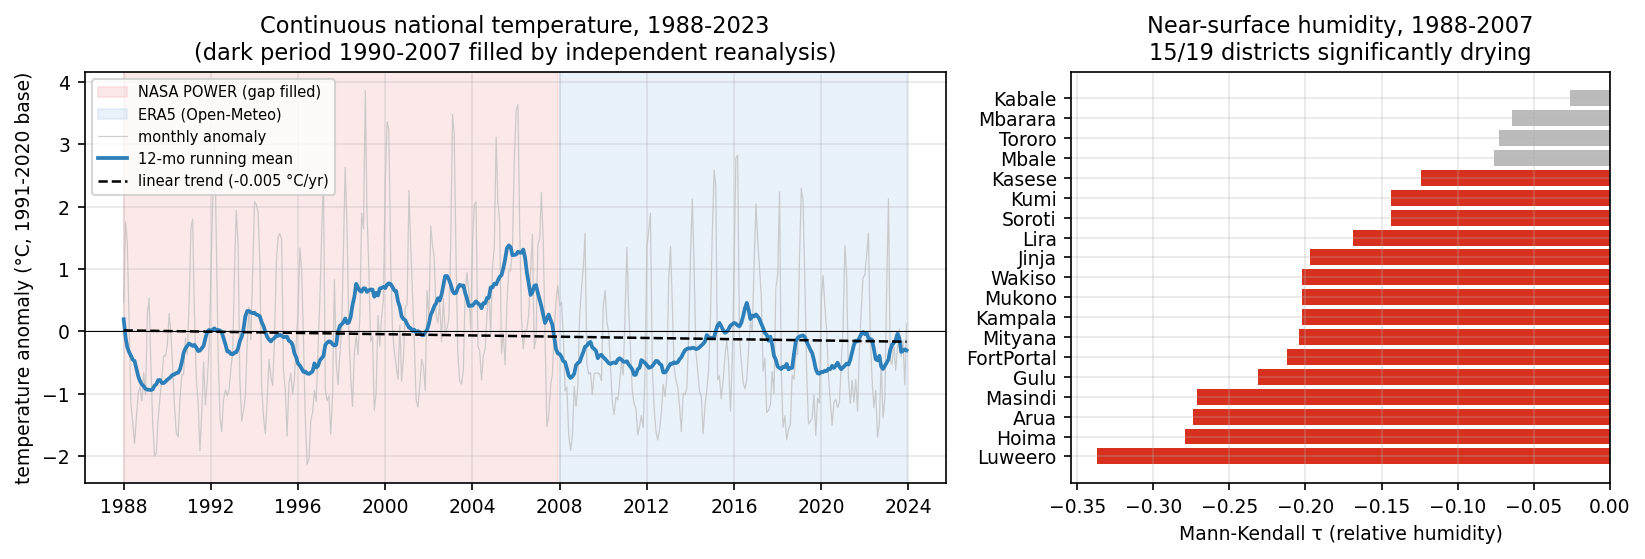
\includegraphics[width=\linewidth]{figures/fig_gapfill.png}
\caption{Independent NASA POWER gap-fill. Left: continuous national temperature
anomaly 1988--2023, with the 1990--2007 reporting collapse filled by POWER
(shaded). Right: district Mann--Kendall $\tau$ for near-surface humidity over
1988--2007; 15/19 districts dry significantly. (Novel gap-fill)}
\label{fig:gapfill}
\end{figure}
\begin{figure}[h]\centering
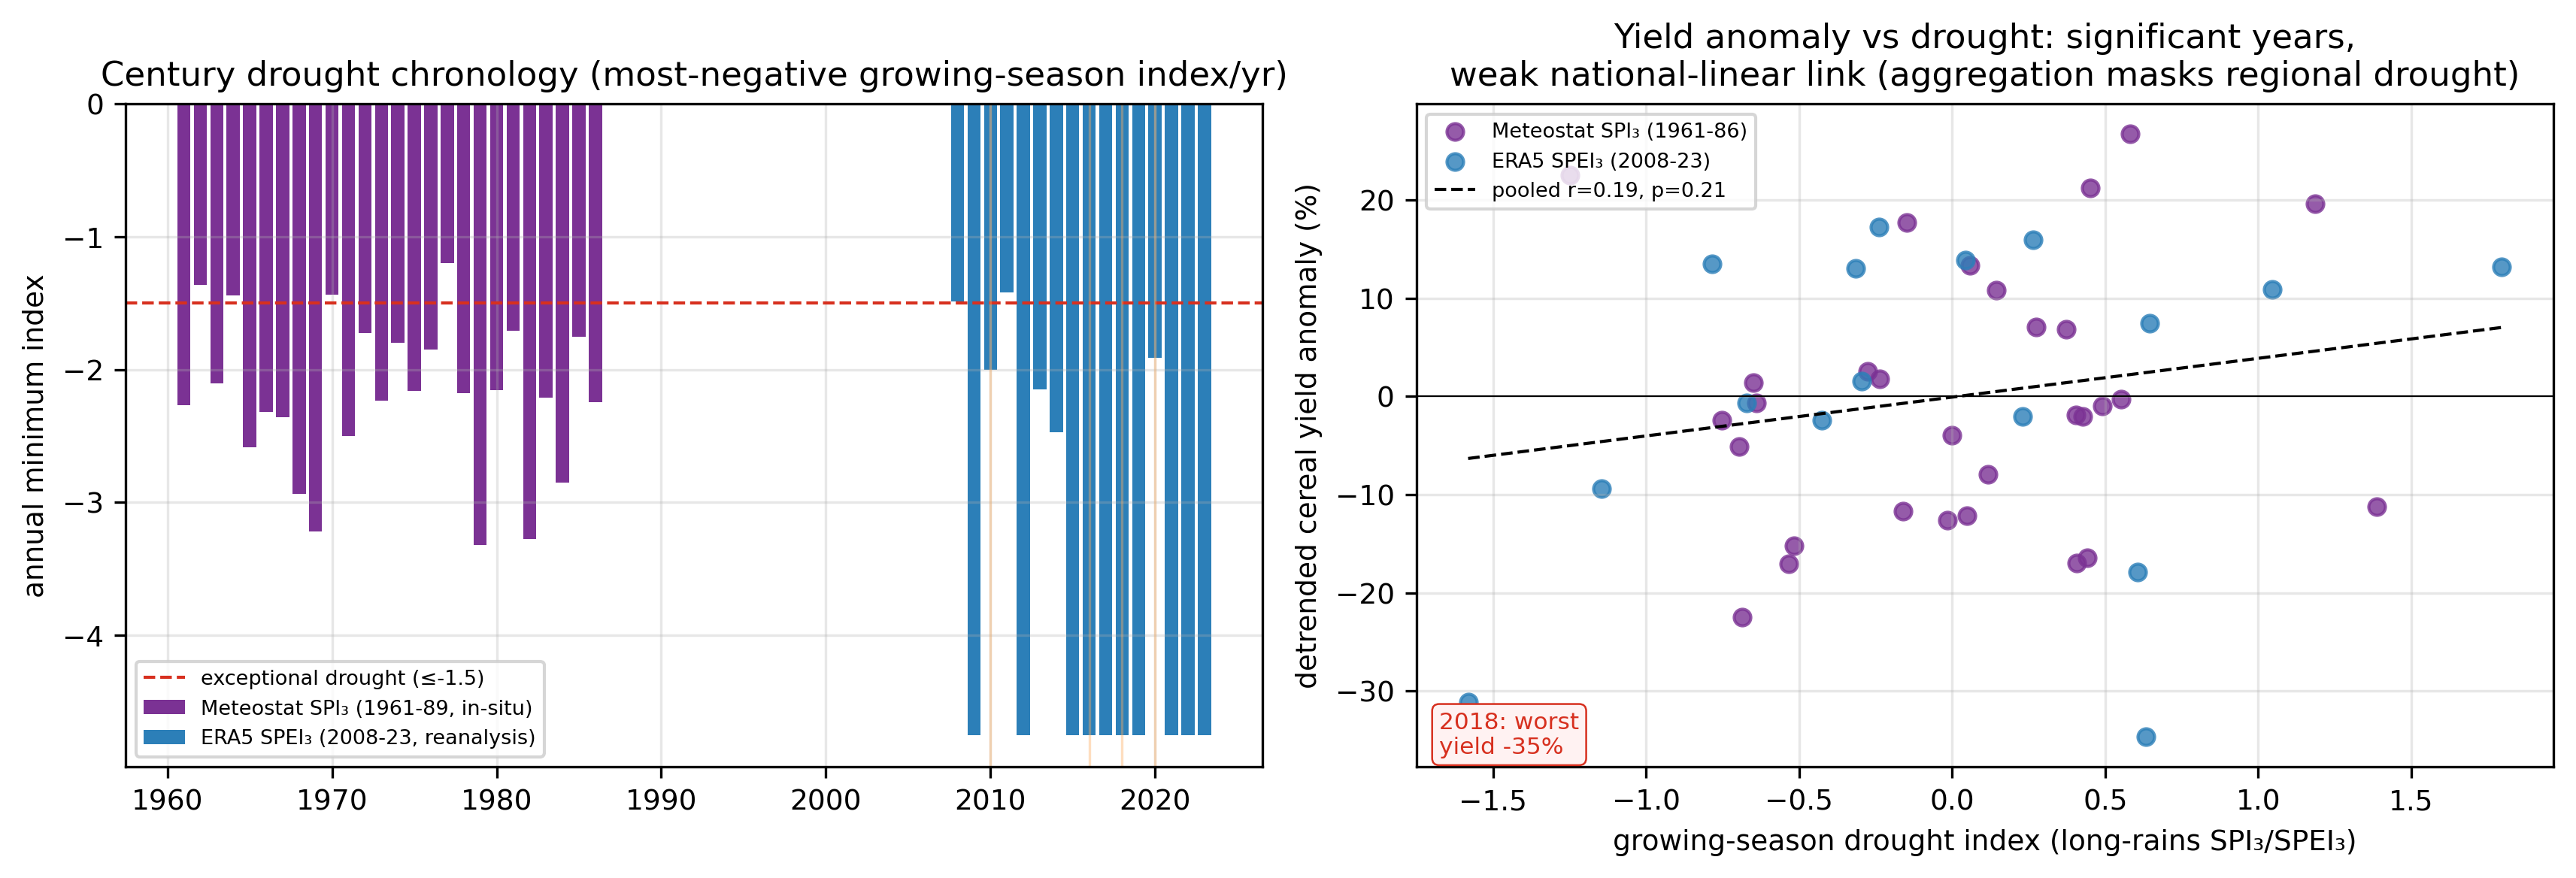
\includegraphics[width=\linewidth]{figures/fig_drought_yield.png}
\caption{Century drought chronology (Meteostat SPI$_3$ 1961--89 and ERA5
SPEI$_3$ 2008--23, most-negative growing-season value per year, with the
1990--2007 in-situ gap visibly empty) and detrended cereal-yield anomaly versus
growing-season drought index, showing significant drought--yield years but a
weak national-linear link. (Drought $\rightarrow$ impact)}
\label{fig:droughtyield}
\end{figure}
\begin{figure}[h]\centering
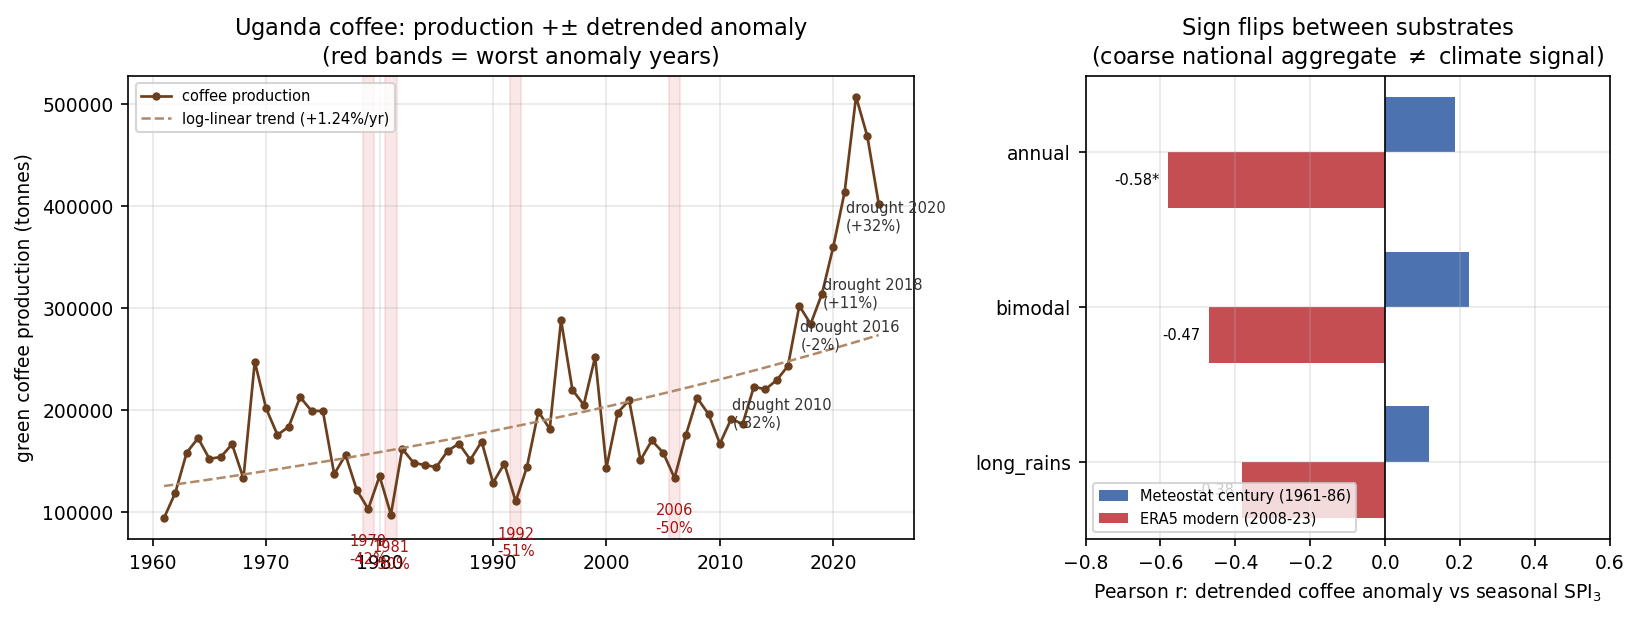
\includegraphics[width=\linewidth]{figures/fig_coffee.png}
\caption{Uganda coffee: the confounding generalises to the signature export.
Left: green-coffee production (t) 1961--2024 with the fitted log-linear trend
($+1.24\%$/yr), worst detrended-anomaly years banded, and documented drought
years annotated (2018 and 2020 are record harvests, not losses). Right: Pearson
$r$ of the production anomaly against seasonal SPI$_3$ on two independent
substrates: weak-positive on the century in-situ record, negative (and
marginally significant, $*$) on modern ERA5. The sign flip shows a coarse
national crop aggregate carries no stable climate signal. (Coffee impact)}
\label{fig:coffee}
\end{figure}
\begin{figure}[h]\centering
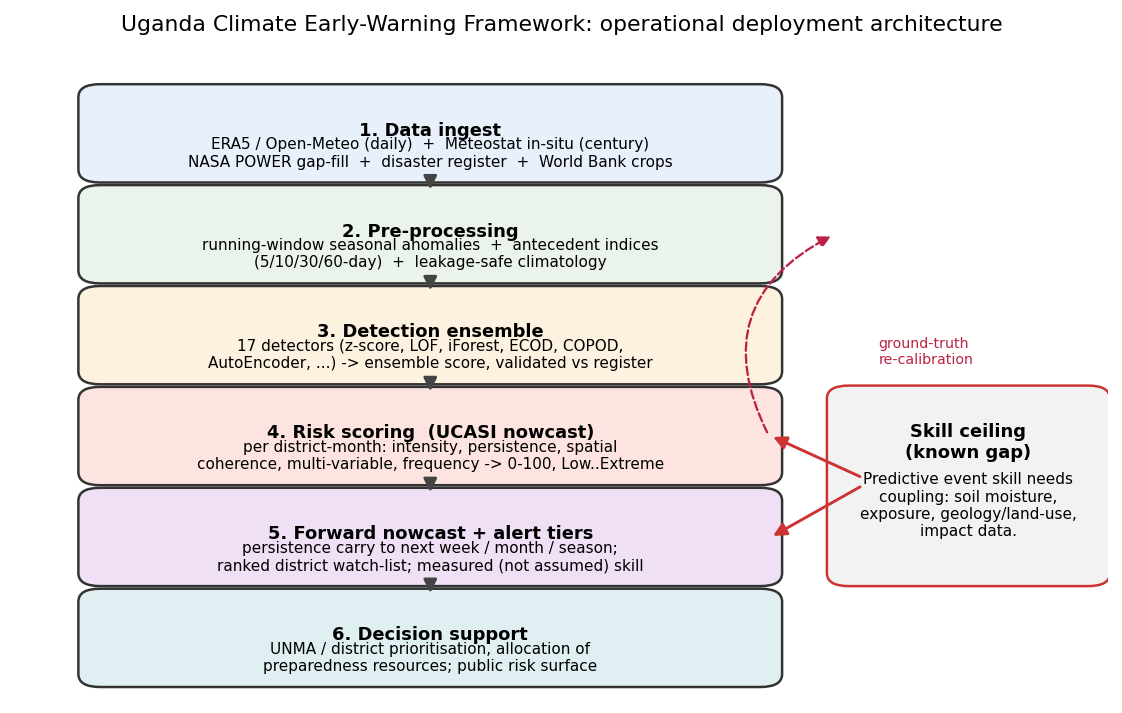
\includegraphics[width=\linewidth]{figures/fig_ews_architecture.png}
\caption{Operational deployment architecture of the Uganda Climate Early-Warning
Framework: six stages from multi-source ingest through leakage-safe
pre-processing, the validated detection ensemble, the UCASI district-month risk
nowcast, a persistence-based forward carry with alert tiers, and decision
support. The dashed edge is ground-truth re-calibration against the register; the
red box marks the measured skill ceiling: predictive event skill requires
coupling exposure, soil moisture and impact data absent from a weather-only
feature space.}
\label{fig:architecture}
\end{figure}
\begin{figure}[h]\centering
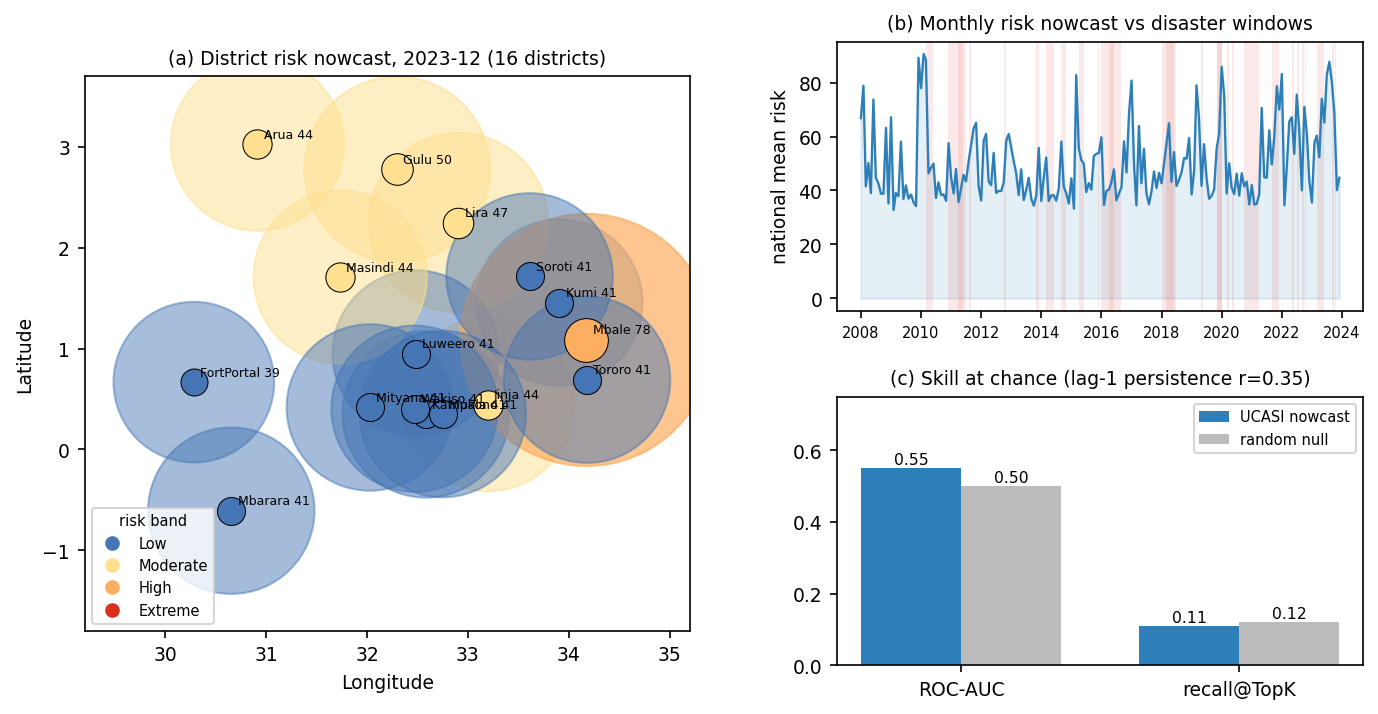
\includegraphics[width=\linewidth]{figures/fig_risk_nowcast.png}
\caption{UCASI forward risk nowcast. (a) District risk surface for the most recent
month: bubble size/colour encode the 0--100 score and severity band; Mbale (78,
High) leads with the northern belt Moderate. (b) National monthly mean risk
2008--2023 with documented disaster windows shaded. (c) Honest skill: the
district-month score is at chance against a size-matched random null (ROC-AUC
$0.55$ vs $0.50$; recall@TopK $0.11$ vs $0.12$), and the forward carry rests on
lag-1 persistence ($r=0.35$), not predictive power.}
\label{fig:nowcast}
\end{figure}

%============================================================================
\bibliographystyle{elsarticle-num}
\bibliography{references}

\end{document}
